%% Chapter 2 — Virtualization Principles and Cloud Compute
\setcounter{chapter}{1}
\chapter{Virtualization Principles and Cloud Compute}
\chaptersubtitle{What really happens when you "rent a GPU VM" — from CPU modes to microVMs to MIG}

\begin{calloutbox}{tbbblue}{tbbbluefill}
{\normalsize\bfseries\color{tbbblue}Learning objectives}\par\vspace{3pt}
\begin{tbbitemize}
  \item Interrogate a rented cloud VM (\code{dmidecode}, \code{systemd-detect-virt}, \code{kvm-clock}) and read the evidence that it does not physically exist — then retell the sixty-year utilization story (million-dollar mainframes → the 2000s' empty servers → EC2's \$0.10 hour) that explains why the industry keeps rebuilding this illusion.
  \item State Popek and Goldberg's three requirements for a virtual machine monitor, explain why classic x86 failed them, and describe the two software workarounds (binary translation and paravirtualization) that carried the industry until 2005.
  \item Explain hardware-assisted virtualization — VMX root/non-root modes, the VMCS, VM exits, and EPT/NPT — and use "number and cost of exits" as a lens for virtualization performance.
  \item Describe how KVM, QEMU, and virtio divide the work of running a VM on Linux, and why a paravirtual device is faster than an emulated one.
  \item Place processes, containers, gVisor, microVMs, and full VMs on the isolation spectrum, and argue which point fits a given multi-tenant workload — including why AWS built Firecracker for Lambda.
  \item Compare the three ways a GPU reaches a workload — PCIe passthrough, vGPU/time-slicing, and MIG — and their consequences for performance isolation and cost.
  \item Launch, benchmark (CPU vs. GPU inference), and safely shut down your first cloud GPU VM, with billing guardrails in place before anything else.
\end{tbbitemize}
\end{calloutbox}

\vspace{5.0pt}

\begin{calloutbox}{tbbteal}{tbbtealfill}
{\normalsize\bfseries\color{tbbteal}Key terms}\par\vspace{3pt}
time-sharing (CP-67 / VM) · server sprawl · utilization · hypervisor / VMM · Type 1 vs. Type 2 · trap-and-emulate · sensitive vs. privileged instructions · binary translation · paravirtualization · VT-x / AMD-V · VMX root/non-root · VMCS · VM exit · EPT / NPT · KVM · QEMU · vCPU · steal time · virtio · virtqueue · vhost · SR-IOV · IOMMU (VT-d) · microVM · Firecracker · gVisor · Kata Containers · PCIe passthrough (VFIO) · vGPU · time-slicing · MPS · MIG
\end{calloutbox}

\vspace{5.0pt}

\begin{calloutbox}{tbblightgray}{tbbboxfill}
{\normalsize\bfseries\color{tbbink}Chapter outline}\par\vspace{3pt}
\textbf{2.1} The machine you rented doesn't exist    \textbf{2.2} Hypervisors and the trapping problem    \textbf{2.3} Hardware-assisted virtualization: VT-x, VMCS, and EPT    \textbf{2.4} KVM, QEMU, and virtio: Linux as the cloud's hypervisor    \textbf{2.5} How small can a VM get? microVMs and the isolation spectrum    \textbf{2.6} GPUs in the cloud: instances, passthrough, and sharing    \textbf{2.7} Lab: your first cloud GPU — safely — followed by a summary, exercises, and further reading.
\end{calloutbox}

\section{The Machine You Rented Doesn't Exist}

At some point this week you will click a button labeled \textbf{Launch instance}, wait perhaps forty seconds, and then ssh into "your" machine. It will have a hostname, CPUs, memory, a disk, and — for the first time in this course — a GPU. You can reboot it. You can break it. It behaves in every way like a computer that belongs to you.

Here is the uncomfortable truth this chapter unpacks: \textbf{that computer does not exist.} No human racked a server when you clicked the button. Somewhere in a data center there is a very large physical machine — perhaps 128 cores and two terabytes of RAM — running dozens of guests like yours side by side, each convinced it owns the hardware. The software that maintains this illusion is the \textbf{hypervisor}, also called a \textbf{virtual machine monitor (VMM)}, and the illusion itself is a \textbf{virtual machine (VM)}: a faithful, isolated, software-defined replica of a physical computer.

\subsection*{Exhibit A: interrogate the machine}

Strong claims deserve evidence, and this one convicts itself in six commands. The machine keeps its true nature on file — you only have to ask:

\begin{terminalbox}
\begin{Verbatim}[breaklines=true,breakanywhere=true,fontsize=\small,formatcom=\color{tbbtermfg},codes=\tbbcodeactive]
$ ssh ubuntu@203.0.113.7            # "your" machine, forty seconds old
$ sudo dmidecode -s system-manufacturer
Amazon EC2                          # the "manufacturer" is a retailer
$ sudo dmidecode -s system-product-name
g4dn.xlarge                         # the "model number" is a price tag
$ systemd-detect-virt
kvm                                 # the OS knows. it has always known.
$ lscpu | grep Hypervisor
Hypervisor vendor:   KVM
$ cat /sys/devices/system/clocksource/clocksource0/current_clocksource
kvm-clock                           # even TIME arrives via the hypervisor
$ nvidia-smi -L
GPU 0: Tesla T4 (UUID: GPU-8f61c81e...)   # and yet THIS is physically real
\end{Verbatim}
\end{terminalbox}
\figcaption{Exhibit 2-A  The rented machine, interrogated. Firmware strings, the virtualization detector, the CPU flags, the clock — every layer testifies that the computer is software. Except the last line, which will take Section 2.6 to explain.}

Read the confession line by line. The DMI firmware strings — fields that on a laptop would say \textit{LENOVO} and a model number — hold a retailer's name and a billing SKU, because the hypervisor authored them and saw no reason to lie about \textit{that}. \code{systemd-detect-virt} is not doing anything exotic: the guest can simply ask (a \code{CPUID} leaf reserved for hypervisors — Section 2.3 explains who answers it). Even the clock is a paravirtual service, because a guest that gets descheduled cannot keep honest time alone (\code{kvm-clock} — and its cousin \textit{steal time} — return in Section 2.4 with your p99 attached). And then the last line refuses the pattern: the disk is virtual, the NIC is virtual, time itself is virtual — but the T4 is \textbf{a real card, passed through whole}. A machine that is entirely fake except for its most expensive component is a strange artifact; by Section 2.6 you will know exactly why the industry builds it that way.

\subsection*{Exhibit B: the empty machines}

Why does this illusion exist at all? Not for elegance — for \textbf{money}, twice over, fifty years apart. The story is worth three paragraphs because, as you will see, this course lives inside its third act.

\textbf{Act one: the machine costs millions (1960s).} A mainframe of the era cost several million dollars and, run as its makers first intended — one job at a time — idled between jobs while humans shuffled tapes. The economic pressure to \textit{slice one precious machine among many users} produced time-sharing, and at IBM's Cambridge lab it produced something stranger and more durable: \textbf{CP-67 (1967)}, software that gave every user not a login session but \textit{an entire simulated System/360 of their own}, each running its own single-user OS. Virtualization was not invented for the cloud; it was invented because hardware was expensive and idle — and it is older than UNIX.

\textbf{Act two: the machines are empty (2000s).} Fast-forward: servers are now cheap enough that enterprises buy one per application — partly manageability, partly superstition ("the mail server and the database \textit{will} fight"). The result was \textbf{server sprawl}: racks of beige boxes, surveys of the era putting typical utilization at \textbf{5–15\%} — corporate data centers as, in effect, warehouses full of idle CPUs, each burning power and cooling. Onto x86 (which, as Section 2.2 explains, resisted virtualization on a technicality) VMware brought the 1960s trick back (1999–2001), and \textit{consolidation} — ten mostly-idle machines folded into one — sold itself: the ROI case was literally "delete nine electric bills."

\textbf{Act three: the meter (2006).} On August 25, 2006, Amazon opened a beta of something called Elastic Compute Cloud: virtual machines for rent over an API, the small size priced at \textbf{\$0.10 per hour}. The consequential word was not \textit{cloud} but \textit{hour}: allocation had become a software operation (this chapter's subject), so compute could be metered like electricity — no procurement, no racking, no minimum. Every economic structure Chapter 1 taught — hourly GPU pricing, per-token APIs, serverless billing, Exhibit 1-B's \$779 lesson included — descends from that meter. And here is the symmetry that makes the story ours: \textbf{the GPU is now living act one again.} An H100 is this decade's million-dollar mainframe — brutally expensive, chronically under-shared — and Section 2.6's passthrough → time-slicing → MIG is the same journey (exclusive use → software sharing → hardware partitions) the CPU took across these three acts, replayed on silicon. Architecture rhymes; this chapter teaches you the rhyme scheme.

Chapter 1 asked you to take "rent a GPU VM" on faith. This chapter opens the box, because the mechanism inside is not a detail — it is the foundation on which every topic in this course stands. Four reasons, up front.

\subsection*{Why the cloud is built on virtualization}

\textbf{First: utilization economics.} Recall from Chapter 1 that the central cost problem of AI infrastructure is expensive hardware sitting idle. A physical server sold whole to one customer idles whenever that customer idles. A physical server carved into virtual machines can host many tenants whose peaks and troughs interleave, so the provider sells the same silicon several times over — and can offer you a slice as small as you want for as long as you want. Per-hour billing, the entire economic premise of Chapter 1's tables, is only possible because allocation is a software operation.

\textbf{Second: isolation between strangers.} Your VM shares a physical machine with tenants you will never meet — possibly your competitors. The hypervisor is the referee that guarantees they cannot read your memory, exhaust your CPU share, or crash your kernel. How strong that referee is, and what it costs in performance, is a running theme of this chapter — and the entire subject of Section 2.5, because the answer changes when workloads shrink from "a rented server" to "a serverless function that lives for 200 milliseconds."

\textbf{Third: elasticity is only a software call away.} Chapter 1 established that inference load is bursty and that the remedy is elastic scaling. Elasticity is physically possible because "creating a machine" means creating a process-like software object, not racking hardware. When we study autoscaling in Week 12, every scale-out event will bottom out in exactly the sequence this chapter explains: allocate, boot, load, serve. The time that sequence takes is the \textbf{cold start} — and its floor is set by virtualization technology, which is why AWS had to invent a new kind of VM (Firecracker, Section 2.5) to make Lambda viable.

\textbf{Fourth: the fleet is heterogeneous; your VM is not.} Providers run generations of hardware side by side. The virtualization layer normalizes this zoo into stable instance types, lets the provider migrate, drain, and patch hosts under running guests, and lets you snapshot a whole machine as a file. Operations that would be hardware projects become API calls.

\subsection*{Why an AI serving engineer should care about the internals}

You could use the cloud for years without knowing what a VMCS is. But this course promised to take you below the abstractions you depend on, and this layer repays the visit unusually well:

\begin{tbbitemize}
  \item \textbf{Your p99 has roots down here.} A vCPU is a thread the host schedules (Section 2.4); on an oversold host your guest experiences "steal time" — invisible pauses that surface as tail-latency spikes no amount of application tuning will fix. Knowing this turns a mystery into a diagnosis.
  \item \textbf{Cold starts are a virtualization problem before they are an ML problem.} Scale-to-zero (Week 12) stands or falls on how fast an isolated execution environment can be conjured. Firecracker's 125-millisecond microVM is the state of the art you will reason about.
  \item \textbf{GPU sharing (Week 12) is applied GPU virtualization.} Whether one H100 can safely serve three tenants is decided by passthrough vs. vGPU vs. MIG — Section 2.6's subject.
  \item \textbf{This week's lab bill is real money.} Understanding what an instance is — and what stop, terminate, and attached storage mean underneath — is the difference between a \$2 lab and a \$200 surprise (Section 2.7).
\end{tbbitemize}

\subsection*{Vocabulary for the chapter}

\begin{tbbtablewrap}
  \begin{tabular}{@{}>{\raggedright\arraybackslash}m{\dimexpr 0.2660\tbltextwidth-2\tabcolsep\relax} >{\raggedright\arraybackslash}m{\dimexpr 0.7340\tbltextwidth-2\tabcolsep\relax}@{}}
  \arrayrulecolor{tbbnavy}\specialrule{1pt}{0pt}{0pt}
  \rowcolor{tbbtablehead}{\centering \bfseries\color{tbbnavy}Term} & {\centering \bfseries\color{tbbnavy}Meaning} \\
  \arrayrulecolor{tbbnavy}\specialrule{0.7pt}{0pt}{2pt}
  {\textbf{virtual machine (VM)}} & {A software-created replica of a physical computer, faithful enough to run an unmodified operating system.} \\
  \arrayrulecolor{tbbtableborder}\hline
  {\textbf{hypervisor / VMM}} & {The software that creates and referees VMs: multiplexes real hardware among guests while keeping them isolated.} \\
  \arrayrulecolor{tbbtableborder}\hline
  {\textbf{host / guest}} & {The physical machine and its operating environment (host) vs. the virtualized environment and OS running inside a VM (guest).} \\
  \arrayrulecolor{tbbtableborder}\hline
  {\textbf{virtualize vs. emulate}} & {Virtualizing runs guest instructions directly on the real CPU whenever safe; emulating interprets them in software (flexible, slow). Hypervisors virtualize the CPU and, classically, emulate devices.} \\
  \arrayrulecolor{tbbtableborder}\hline
  {\textbf{trap}} & {A hardware-forced transfer of control to a more privileged layer when code attempts something it may not do — the basic mechanism the VMM builds on.} \\
  \arrayrulecolor{tbbtableborder}\hline
  {\textbf{VM exit / entry}} & {The hardware switch from guest execution to the hypervisor (exit) and back (entry) under VT-x/AMD-V. The unit of virtualization overhead.} \\
  \arrayrulecolor{tbbtableborder}\hline
  {\textbf{paravirtualization}} & {Letting the guest know it is virtualized and cooperate through an efficient interface, instead of maintaining a perfect illusion. virtio is its modern descendant.} \\
  \arrayrulecolor{tbbtableborder}\hline
  {\textbf{device model}} & {The hypervisor component that impersonates hardware devices (NICs, disks) to the guest — QEMU's main job.} \\
  \arrayrulecolor{tbbtableborder}\hline
  {\textbf{microVM}} & {A VM with a minimal device model and direct kernel boot, designed to start in milliseconds and run thousands-per-host (Firecracker, Cloud Hypervisor).} \\
  \arrayrulecolor{tbbtableborder}\hline
  {\textbf{IOMMU (VT-d / AMD-Vi)}} & {Hardware that translates and polices device DMA, making it safe to hand a physical device (like a GPU) directly to a guest.} \\
  \arrayrulecolor{tbbnavy}\specialrule{1pt}{2pt}{0pt}
  \end{tabular}\par
  \figcaption{Table 2-1  Working vocabulary for this chapter}
\end{tbbtablewrap}

\begin{calloutbox}{tbbpurple}{tbbpurplefill}
{\normalsize\bfseries\color{tbbpurple}Think About It}\par\vspace{3pt}
\begin{tbbitemize}
  \item Run Exhibit 2-A's commands on a physical Linux machine (or WSL2 — and predict first what WSL2 will report, and why that answer is itself interesting). Which lines differ, and what does each difference prove?
  \item Your cloud VM reports 4 vCPUs. List three ways this could be physically realized on the host, and what each would mean for your inference latency. (Revisit after Section 2.4.)
  \item A provider could skip virtualization and rent whole physical servers ("bare metal" offerings do exist). What becomes harder for the provider, and what becomes better for the customer? Who chooses bare metal, and why?
  \item Extend Exhibit 2-B's "the GPU is living act one again" analogy: what would the GPU's act three — its 2006, its meter — look like? Do today's serverless GPU platforms (Chapter 1) qualify, or is something still missing?
\end{tbbitemize}
\end{calloutbox}

\section{Hypervisors and the Trapping Problem}

A hypervisor's job description sounds impossible on first reading: run a complete, unmodified operating system — software written to own a machine — as an unprivileged tenant, without it noticing and without it being able to escape. That this works at all rests on one old, elegant idea; that it works \textit{fast} rests on a hardware feature you will meet in Section 2.3. Let us build the idea first.

\subsection*{The interposition idea, and Popek \& Goldberg's rules}

An operating system kernel manages hardware through a small set of dangerous actions: switching page tables, disabling interrupts, talking to devices. On a real machine, the CPU's privilege system (on x86: \textbf{rings}, with the kernel in ring 0 and applications in ring 3) ensures only the kernel may perform them. The classic virtualization trick — called \textbf{trap-and-emulate} — is to run the guest's kernel \textit{deprivileged}: guest code executes directly on the real CPU at full speed, but the moment it attempts a dangerous action, the hardware \textbf{traps} to the hypervisor, which performs an equivalent-but-safe operation on the guest's virtual view of the machine (its virtual interrupt state, its virtual page tables, its virtual devices) and resumes the guest. The guest ran on real silicon almost the whole time, yet never actually touched the real machine's controls.

In 1974 — decades before the cloud — Gerald Popek and Robert Goldberg formalized when this trick can work, in a paper whose vocabulary we still use.

\begin{calloutbox}{tbbblue}{tbbbluefill}
{\normalsize\bfseries\color{tbbblue}Box 2-1  Popek \& Goldberg (1974): what a real VMM must provide}\par\vspace{3pt}
\begin{tbbitemize}
  \item \textbf{Equivalence (fidelity).} Software running in the VM behaves essentially identically to running on real hardware. The guest OS must not need to be told.
  \item \textbf{Efficiency (performance).} The overwhelming majority of guest instructions execute directly on the real CPU with no VMM intervention. This rules out "just interpret everything" — that is emulation, not virtualization.
  \item \textbf{Resource control (safety).} The VMM stays in complete control of physical resources; no guest action can affect resources outside its allocation.
\end{tbbitemize}

And the theorem: a machine can be virtualized this way \textbf{iff every sensitive instruction (one that reads or affects privileged machine state) is also a privileged instruction (one that traps when executed without privilege)}. In other words: everything dangerous must be trappable. — "Formal Requirements for Virtualizable Third Generation Architectures," CACM 1974.
\end{calloutbox}

\vspace{3.0pt}

The theorem gives us a clean mental model: run the guest deprivileged, let dangerous things trap, emulate them in the VMM. Equivalence and resource control come from trapping; efficiency comes from everything else running natively.

\subsection*{The x86 embarrassment: sensitive but not privileged}

There was just one problem: the most important CPU architecture in the world flunked the theorem. A 2000 analysis by Robin and Irvine catalogued \textbf{17 instructions in classic x86 that are sensitive but not privileged} — executed by a deprivileged guest kernel, they neither work correctly \textit{nor} trap. They simply do the wrong thing, silently. Two flavors give the taste:

\begin{tbbitemize}
  \item \code{POPF} restores the CPU flags register, including the interrupt-enable flag — a guest kernel uses it expecting to switch interrupts on or off. Deprivileged, the interrupt bit is \textit{silently ignored}: no trap, no error, and the guest kernel now has a wrong belief about its own interrupt state. Good luck debugging that.
  \item Instructions like \code{SGDT}/\code{SIDT} read privileged table registers \textit{without any privilege check}, leaking real-machine state into the guest and breaking the illusion of equivalence.
\end{tbbitemize}

So pure trap-and-emulate was impossible on x86 — exactly when the dot-com era made server consolidation commercially urgent. The industry produced two heroic workarounds, both worth knowing because their ideas survive inside today's stack.

\subsection*{Workaround one: binary translation (VMware, 1999)}

VMware's insight: if the CPU will not trap the 17 offenders, \textit{rewrite the guest so they never execute.} The VMM scans guest kernel code just before it runs and translates it — mostly copying instructions verbatim, but replacing every sensitive instruction with a safe sequence that enters the VMM. Translated blocks are cached, so hot code is translated once and thereafter runs at near-native speed. User-mode guest code, which contains no sensitive instructions worth worrying about, runs untouched. The result satisfied Popek \& Goldberg's spirit on hardware that violated its letter: \textbf{full virtualization} — unmodified guests — via just-in-time surgery on the instruction stream. The engineering was formidable (self-modifying code, precise exceptions, translation-cache invalidation) and the memory of it explains much of the industry's gratitude when hardware finally fixed the problem.

\subsection*{Workaround two: paravirtualization (Xen, 2003)}

The Xen project took the opposite road: \textbf{abandon the illusion.} If maintaining equivalence is the expensive part, tell the guest the truth — that it is a guest — and give it an honest, efficient interface to the hypervisor. The guest kernel is \textit{modified at source level}: where it would execute a privileged operation, it instead makes a \textbf{hypercall} (a deliberate call into the hypervisor, the same shape as a syscall). Batched hypercalls replaced storms of traps; performance was excellent. The costs: you need the guest kernel's source (fine for Linux, awkward for Windows), and you must maintain the modifications forever.

Paravirtualization's pure form faded once hardware support arrived, but its central idea — \textit{a guest that knowingly cooperates outperforms a guest that must be fooled} — is alive and central in every cloud VM today. It survives as \textbf{paravirtual devices}: virtio, Section 2.4. And Xen itself carried the early cloud: EC2 launched on Xen in 2006, and AWS only began replacing it (with the KVM-based Nitro system) in 2017.

\subsection*{Type 1 and Type 2 — and where KVM sits}

One more classic distinction, also from the 1970s literature, organizes hypervisors by \textit{where they run} (Figure 2-1). A \textbf{Type 1} (bare-metal) hypervisor is itself the lowest software layer on the machine: VMware ESXi, Microsoft Hyper-V, Xen. Data centers run Type 1 — smallest attack surface, no host OS underneath to schedule against. A \textbf{Type 2} (hosted) hypervisor runs as an application on a normal OS: VirtualBox or VMware Workstation on your laptop — convenient for development, with an extra layer of host-OS scheduling below your VMs.

\begin{tbbfigure}
  \adjustbox{max width=0.94\linewidth,max totalheight=0.46\textheight}{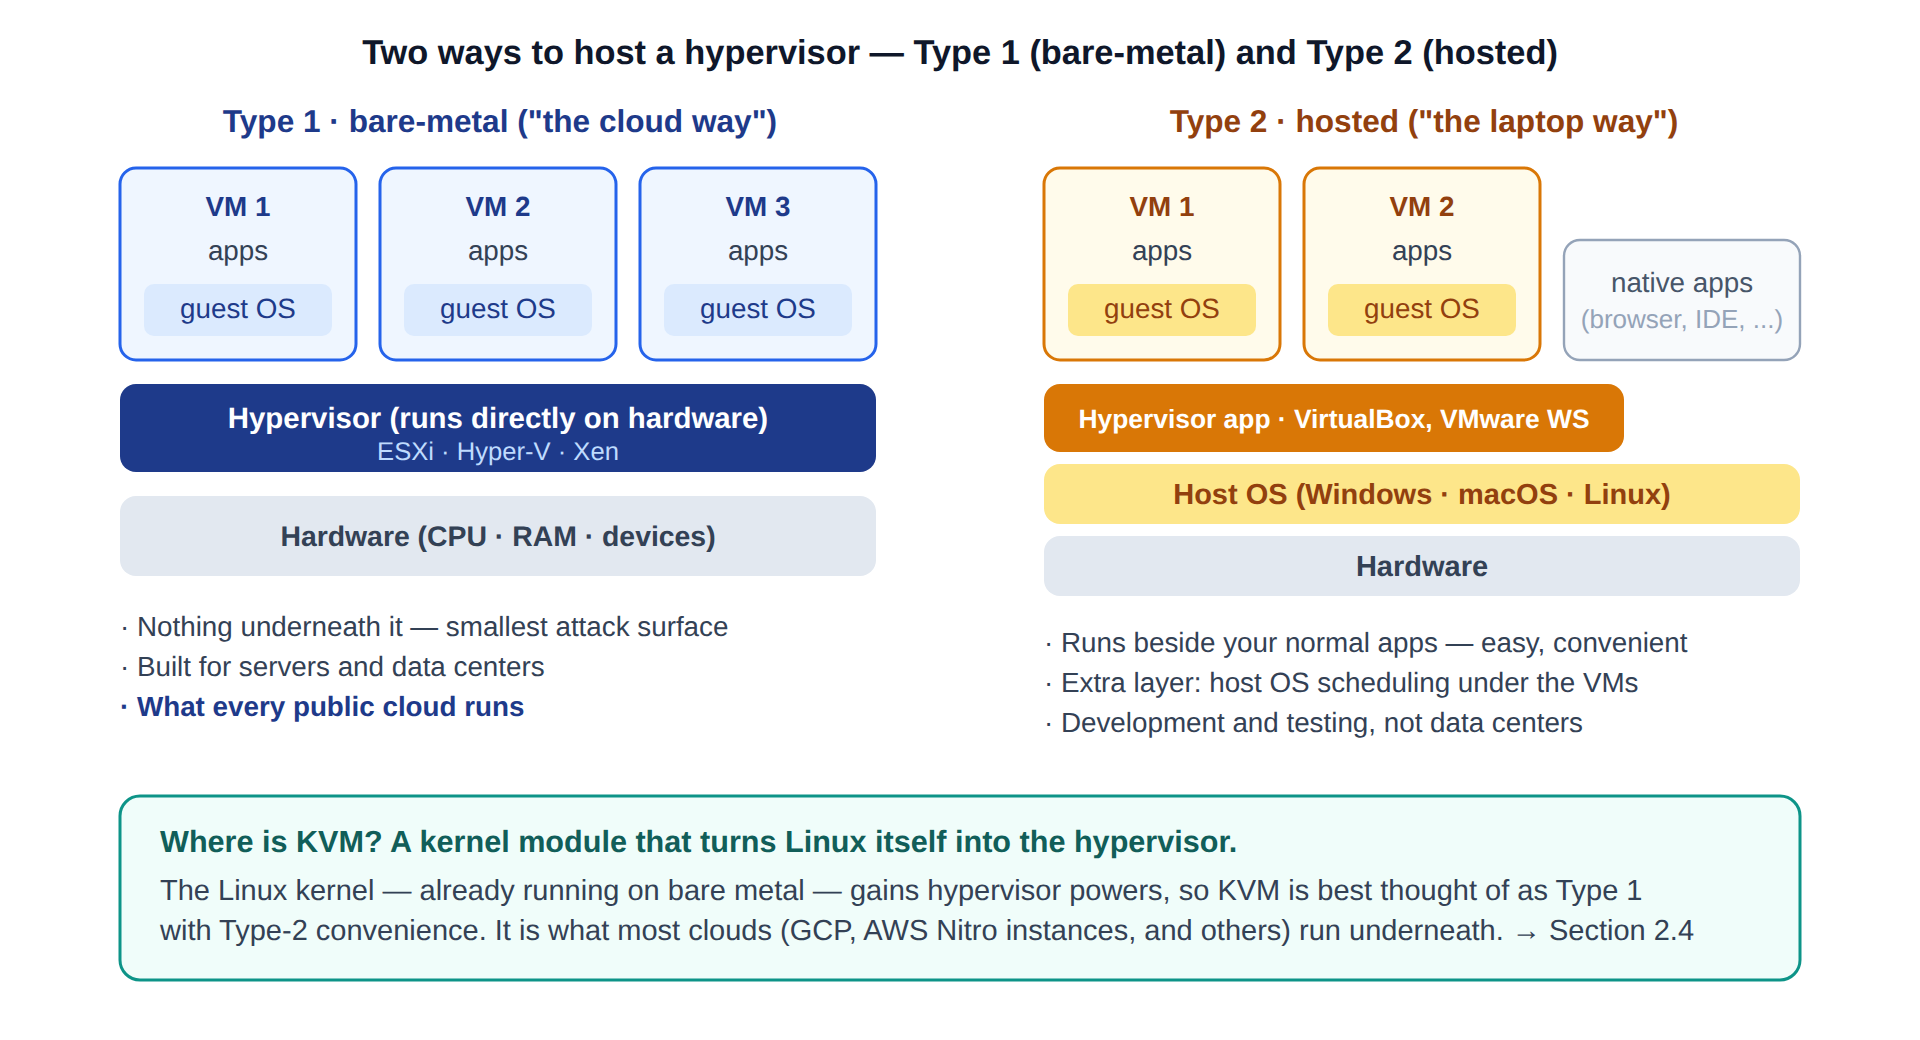
\includegraphics{figures/fig2-1_hypervisors.png}}\\[3pt]
  \figcaption{Figure 2-1  Type 1 (bare-metal) vs. Type 2 (hosted) hypervisors. KVM blurs the line: a kernel module that turns the already-bare-metal Linux kernel into the hypervisor.}
\end{tbbfigure}

The most important hypervisor in the world resists the binary: \textbf{KVM} is a Linux kernel module, so "the host OS" and "the hypervisor" become the same thing — Linux itself, already running on bare metal, gains VMM powers. The pragmatic classification is \textit{Type 1 with Type 2 ergonomics}: hypervisor-grade architecture, but your VMs are managed like ordinary Linux processes with ordinary Linux tools. That combination — plus being open source — is why KVM underlies Google Cloud, modern AWS (Nitro), OpenStack clouds, and this chapter's Section 2.4.

\begin{calloutbox}{tbbpurple}{tbbpurplefill}
{\normalsize\bfseries\color{tbbpurple}Think About It}\par\vspace{3pt}
\begin{tbbitemize}
  \item Classify: a MacBook running Docker Desktop's Linux VM; a GCP host; Windows with WSL2 (hint: WSL2 runs on Hyper-V, and Hyper-V slides \textit{under} the running Windows). Which type is each, and does the question even have a clean answer?
  \item Binary translation preserved equivalence at the cost of complexity; paravirtualization sacrificed equivalence for speed. State one modern situation where each trade is still the right one.
\end{tbbitemize}
\end{calloutbox}

\section{Hardware-Assisted Virtualization: VT-x, VMCS, and EPT}

In 2005–2006, Intel and AMD did what software had been contorting itself to avoid: they changed the processor. Intel's \textbf{VT-x} and AMD's \textbf{AMD-V} made x86 finally satisfy Popek \& Goldberg — not by fixing the 17 instructions one by one, but by giving the CPU an entirely new dimension of privilege. Before the theory, look for the fix on real machines — it is one \code{grep} away:

\begin{terminalbox}
\begin{Verbatim}[breaklines=true,breakanywhere=true,fontsize=\small,formatcom=\color{tbbtermfg},codes=\tbbcodeactive]
# on any modern laptop / workstation running Linux:
$ grep -m1 -c -E "vmx|svm" /proc/cpuinfo
1                          # vmx = Intel VT-x, svm = AMD-V. 2005's fix.
$ ls -l /dev/kvm
crw-rw---- 1 root kvm 10, 232 Jul  6 09:14 /dev/kvm
#   ^ the kernel offering hypervisor powers as a device file (sec. 2.4)

# now the same two commands on this week's rented EC2 guest:
$ grep -m1 -c -E "vmx|svm" /proc/cpuinfo
0                          # the flag is gone. and /dev/kvm does not exist.
# the hypervisor HID it: your guest may not host guests of its own.
# the illusion, by default, refuses to nest.
\end{Verbatim}
\end{terminalbox}
\figcaption{Transcript 2-1  Hunting for VT-x. Your physical laptop advertises vmx/svm and exposes /dev/kvm; inside the rented VM, the hypervisor masks the feature — one CPUID bit, chosen by the VMCS you are about to meet.}

\subsection*{Two worlds: VMX root and non-root mode}

VT-x adds a mode switch \textit{orthogonal} to the rings (Figure 2-2). The hypervisor runs in \textbf{VMX root mode} — the real machine, full control, its own rings 0–3. Guests run in \textbf{VMX non-root mode} — a hardware-supervised world that \textit{also} has rings 0–3. Read that twice, because it dissolves the old dilemma: \textbf{the guest kernel runs in ring 0 again}, exactly as it was written to, so the ugly ring-compression tricks disappear. Non-root ring 0 is simply not the real ring 0: the CPU itself watches guest execution, and on any operation the hypervisor has flagged as intervention-worthy, the hardware performs a \textbf{VM exit} — an automatic, complete world switch into root mode. Handling done, the hypervisor executes a \textbf{VM entry} and the guest resumes, none the wiser. Trap-and-emulate, at last, with the \textit{hardware} doing the trapping — and the 17 embarrassments trap like everything else.

\begin{tbbfigure}
  \adjustbox{max width=0.94\linewidth,max totalheight=0.46\textheight}{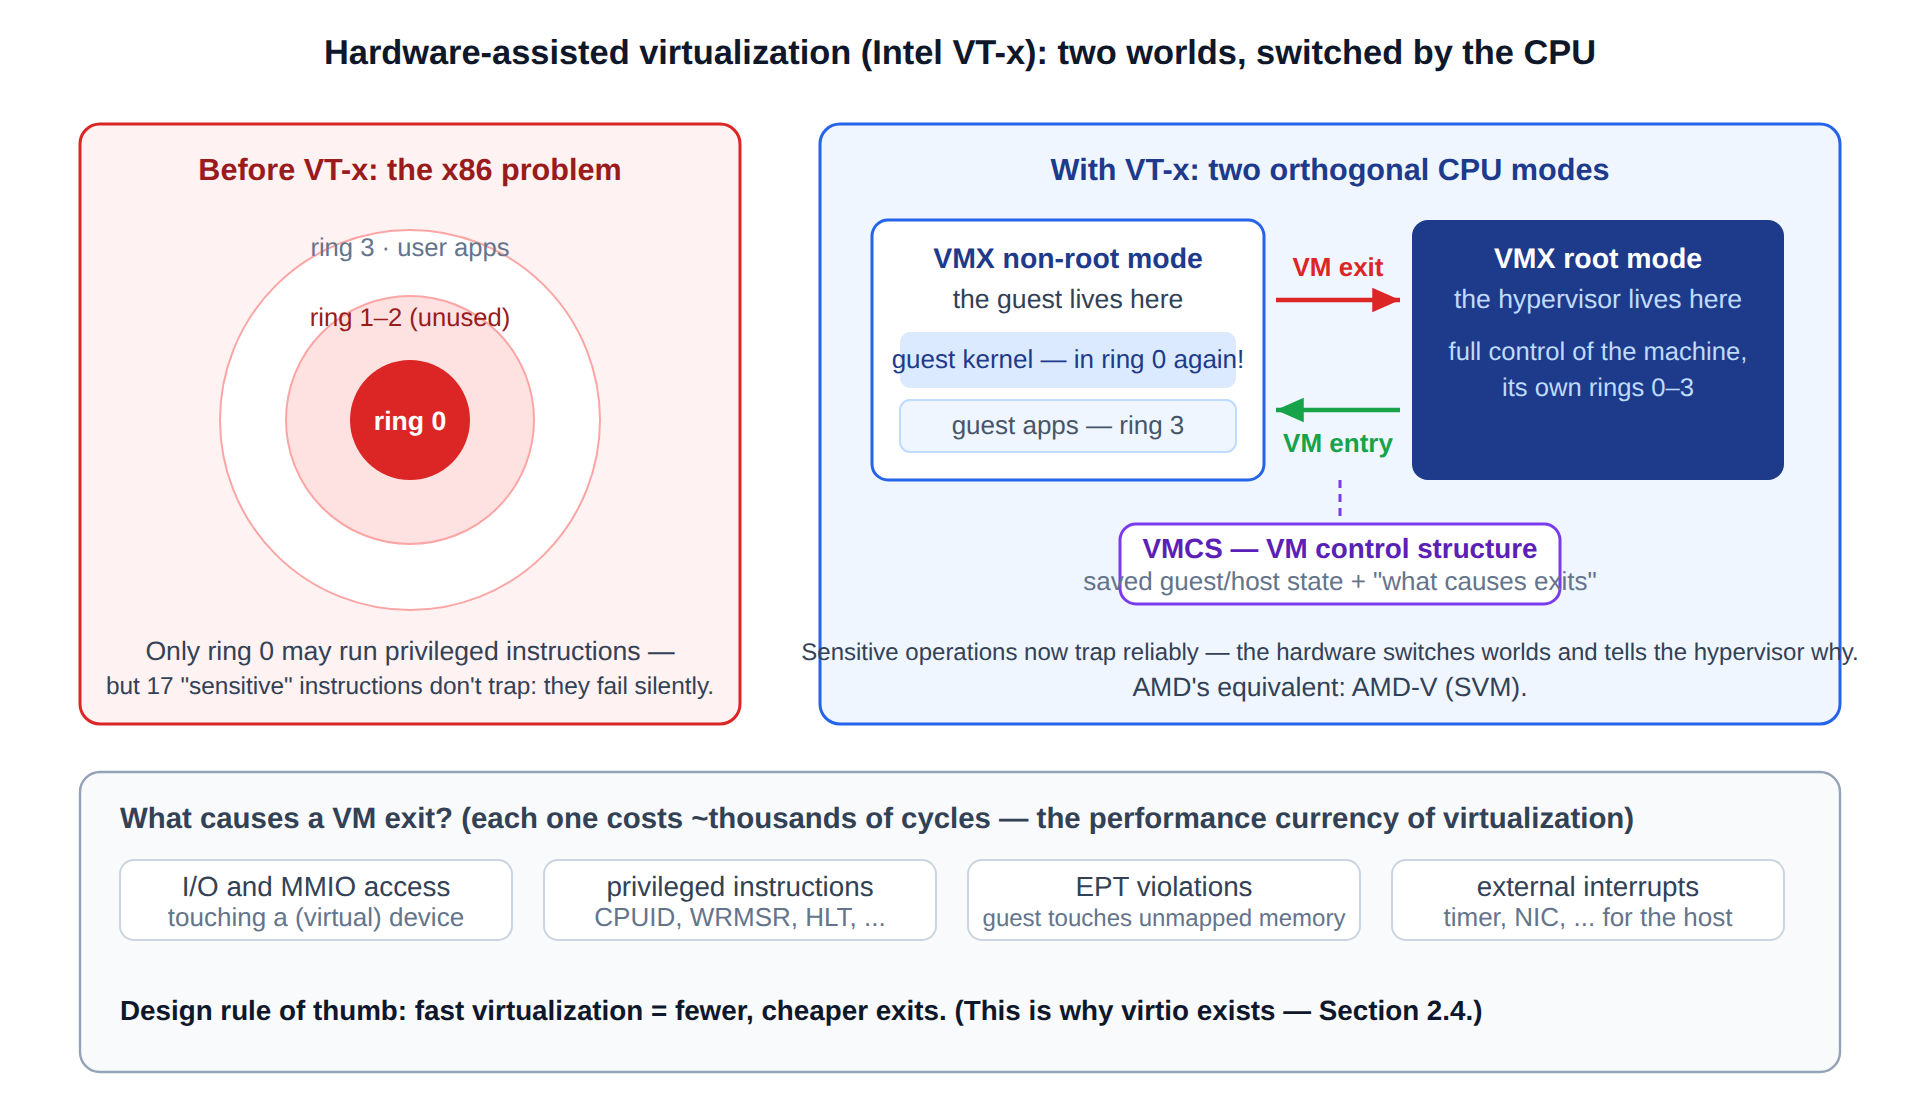
\includegraphics{figures/fig2-2_vtx.png}}\\[3pt]
  \figcaption{Figure 2-2  VT-x in one picture. Left: the pre-2005 problem — deprivileged guest kernels and instructions that fail silently. Right: root/non-root modes, VM exits and entries, and the VMCS that records the rules and the state.}
\end{tbbfigure}

\subsection*{The VMCS: the contract between worlds}

Every world switch needs somewhere to keep the two worlds' states — and the rules of engagement. That is the \textbf{VMCS (Virtual Machine Control Structure)}: one per virtual CPU, holding (a) the guest's register state, loaded on entry and saved on exit; (b) the host's state, restored on exit; and (c) \textbf{control fields} through which the hypervisor programs the hardware: \textit{which} events cause exits (should \code{CPUID} exit? every I/O port access? writes to this control register?), what the guest's view of certain features should be, and where the exit handler lives. On an exit, the hardware also writes the \textbf{exit reason} into the VMCS — so the hypervisor's core is, quite literally, a big \code{switch} statement over exit reasons. When Section 2.4 shows you KVM's run loop, this is the structure it is driving.

\subsection*{Exits are the currency of virtualization performance}

A VM exit is architecturally heavy: save a world, load a world — roughly on the order of a microsecond round-trip once cache effects are counted, thousands of CPU cycles even in the best case. A guest that exits rarely runs at essentially native speed; a guest that exits constantly crawls. This single sentence organizes two decades of virtualization engineering:

\begin{tbbitemize}
  \item \textbf{Reduce the number of exits.} Let the hardware handle in non-root mode what used to require the hypervisor (EPT below, APICv for interrupts), and design device interfaces that batch work per exit instead of exiting per register write (virtio, Section 2.4).
  \item \textbf{Cheapen the exits that remain.} Successive CPU generations have cut world-switch latency; hypervisors route hot exits through slim kernel paths and leave only rare, complex ones to userspace.
\end{tbbitemize}

Keep the lens for the lab and beyond: when a virtualized workload underperforms mysteriously, a practitioner's first question is \textit{what is exiting, and how often} — and tools like \code{perf kvm stat} on the host answer exactly that, tabulating exits by reason. An "exit storm" is to a VM what a syscall storm is to a process.

\subsection*{The second problem: memory, from shadow pages to EPT}

CPU virtualization was only half the battle. Memory is the other half, because address translation now has \textbf{two layers of lies} (Figure 2-3). The guest OS builds page tables translating guest-virtual to \textbf{guest-physical} addresses — but guest-physical addresses are themselves a fiction; the hypervisor decides where guest pages really live in \textbf{host-physical} memory. The hardware page-table walker, pre-2008, could follow only one set of tables. Something had to merge the two translations.

\begin{tbbfigure}
  \adjustbox{max width=0.94\linewidth,max totalheight=0.46\textheight}{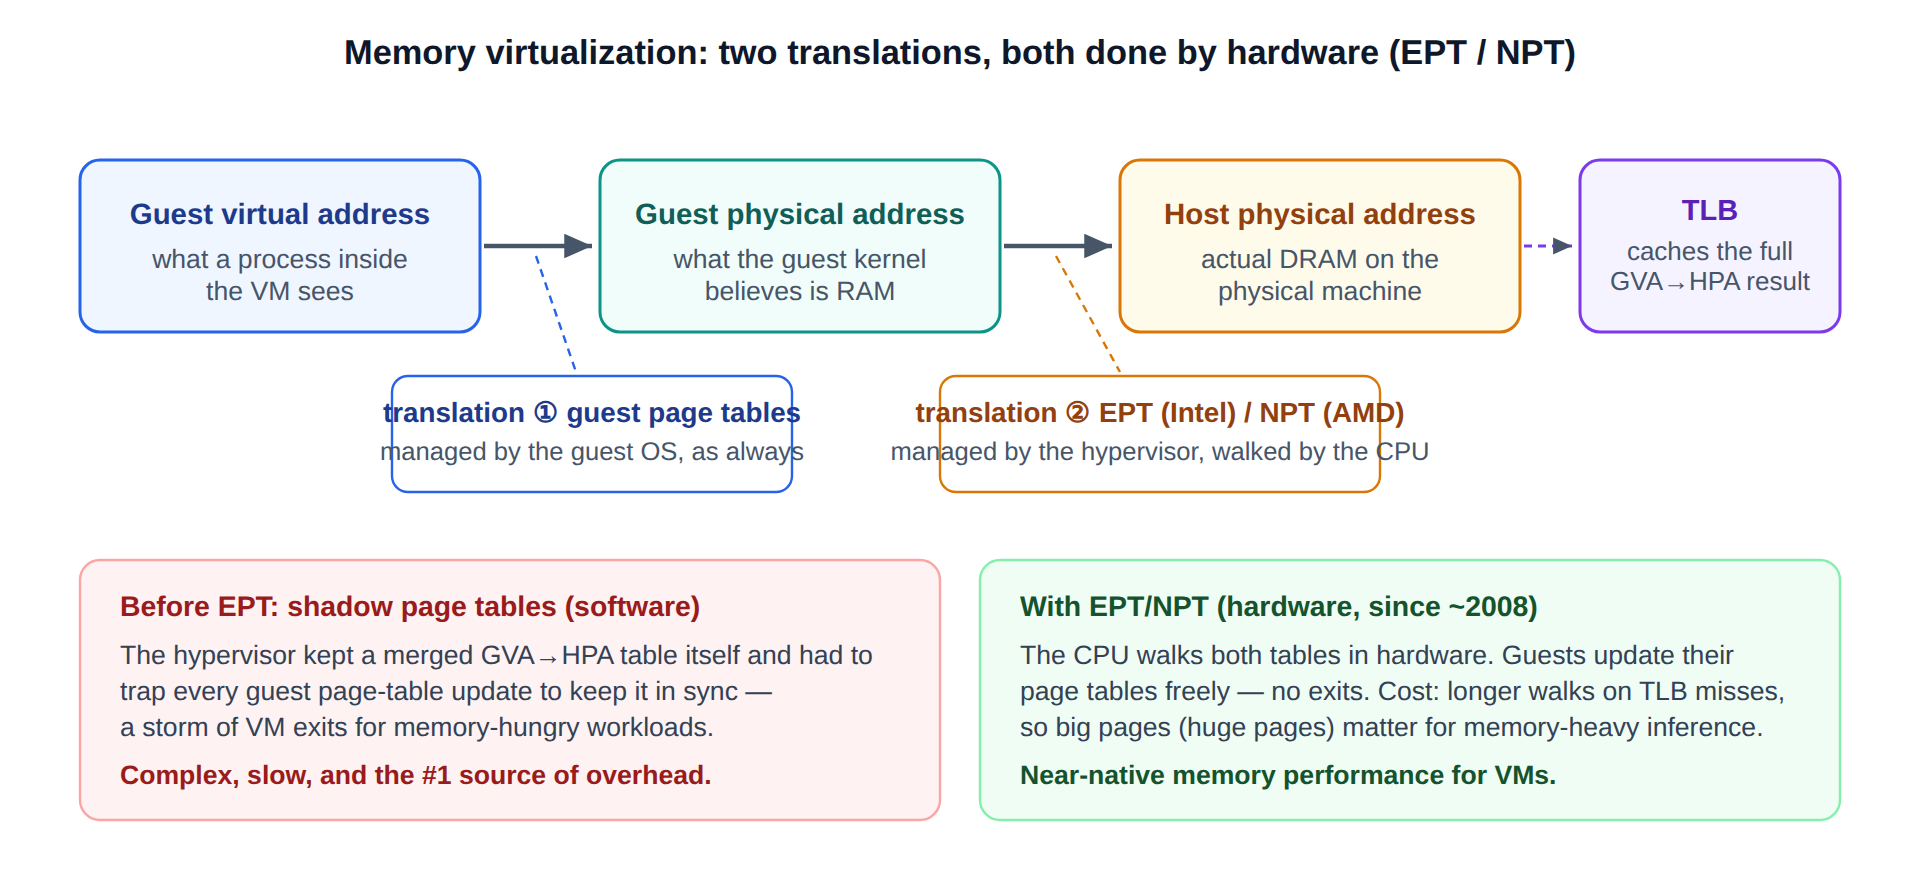
\includegraphics{figures/fig2-3_ept.png}}\\[3pt]
  \figcaption{Figure 2-3  Memory virtualization. Two translations — guest page tables (guest-managed) and EPT/NPT (hypervisor-managed) — both walked by hardware, with the TLB caching the composed result.}
\end{tbbfigure}

The software-era answer was \textbf{shadow page tables}: the hypervisor maintained, for every guest address space, a merged guest-virtual→host-physical table that the real hardware walked — and kept it coherent by write-protecting the guest's page tables and \textbf{trapping every guest page-table update}. For workloads that fork processes or touch memory widely, this meant exit storms and painful slowdowns; shadow paging was the single largest source of virtualization overhead and complexity.

The hardware answer arrived with Intel's \textbf{EPT} (Extended Page Tables, \textasciitilde{}2008) and AMD's \textbf{NPT}: a \textit{second} set of page tables, owned by the hypervisor, that the CPU walks \textit{in addition to} the guest's own. Guest updates its tables freely — no traps, no shadows, no exits. The costs are honest and visible: a TLB miss now requires a two-dimensional walk (in the worst case, each of the 4–5 guest levels needs an EPT walk of its own — up to \textasciitilde{}24 memory references), so \textbf{TLB misses hurt more in a VM}. The standard mitigation is \textbf{huge pages} (2 MB / 1 GB instead of 4 KB), which slash TLB pressure — worth remembering in this course, since inference servers hold multi-gigabyte weight tensors and are exactly the kind of memory-heavy workload that notices. With EPT plus reduced-exit interrupt handling, a well-configured VM's compute and memory performance sits within a few percent of bare metal — which is why the cloud can be built on it.

That settles CPU and memory. The third pillar — \textbf{I/O} — is where the story gets architecturally interesting for us, because it is where Linux, QEMU, and a paravirtual idea called virtio enter. That is the next section.

\begin{calloutbox}{tbbpurple}{tbbpurplefill}
{\normalsize\bfseries\color{tbbpurple}Think About It}\par\vspace{3pt}
\begin{tbbitemize}
  \item Order these guest actions from "exits constantly" to "never exits," and justify: adding two registers; reading a byte from an emulated serial port; a TLB-hit memory load; executing CPUID; updating its own page tables (EPT era).
  \item EPT made guest page-table updates exit-free but made TLB misses costlier. For a 30 GB LLM weight buffer accessed with 4 KB pages vs. 1 GB huge pages, roughly how many TLB entries does each need? What does that suggest?
\end{tbbitemize}
\end{calloutbox}

\section{KVM, QEMU, and virtio: Linux as the Cloud's Hypervisor}

VT-x gave every operating system the raw material for a hypervisor. Linux claimed it almost immediately: \textbf{KVM (Kernel-based Virtual Machine)} was merged into the mainline kernel in early 2007, and its design is a small masterpiece of reuse. Instead of building a new operating system for the hypervisor role — scheduler, memory manager, drivers, all of it — KVM observed that Linux already \textit{had} world-class versions of all three, and simply taught Linux to drive VT-x. The result is the software stack under most of the cloud you will use, and it divides the work three ways (Figure 2-4).

\begin{tbbfigure}
  \adjustbox{max width=0.94\linewidth,max totalheight=0.46\textheight}{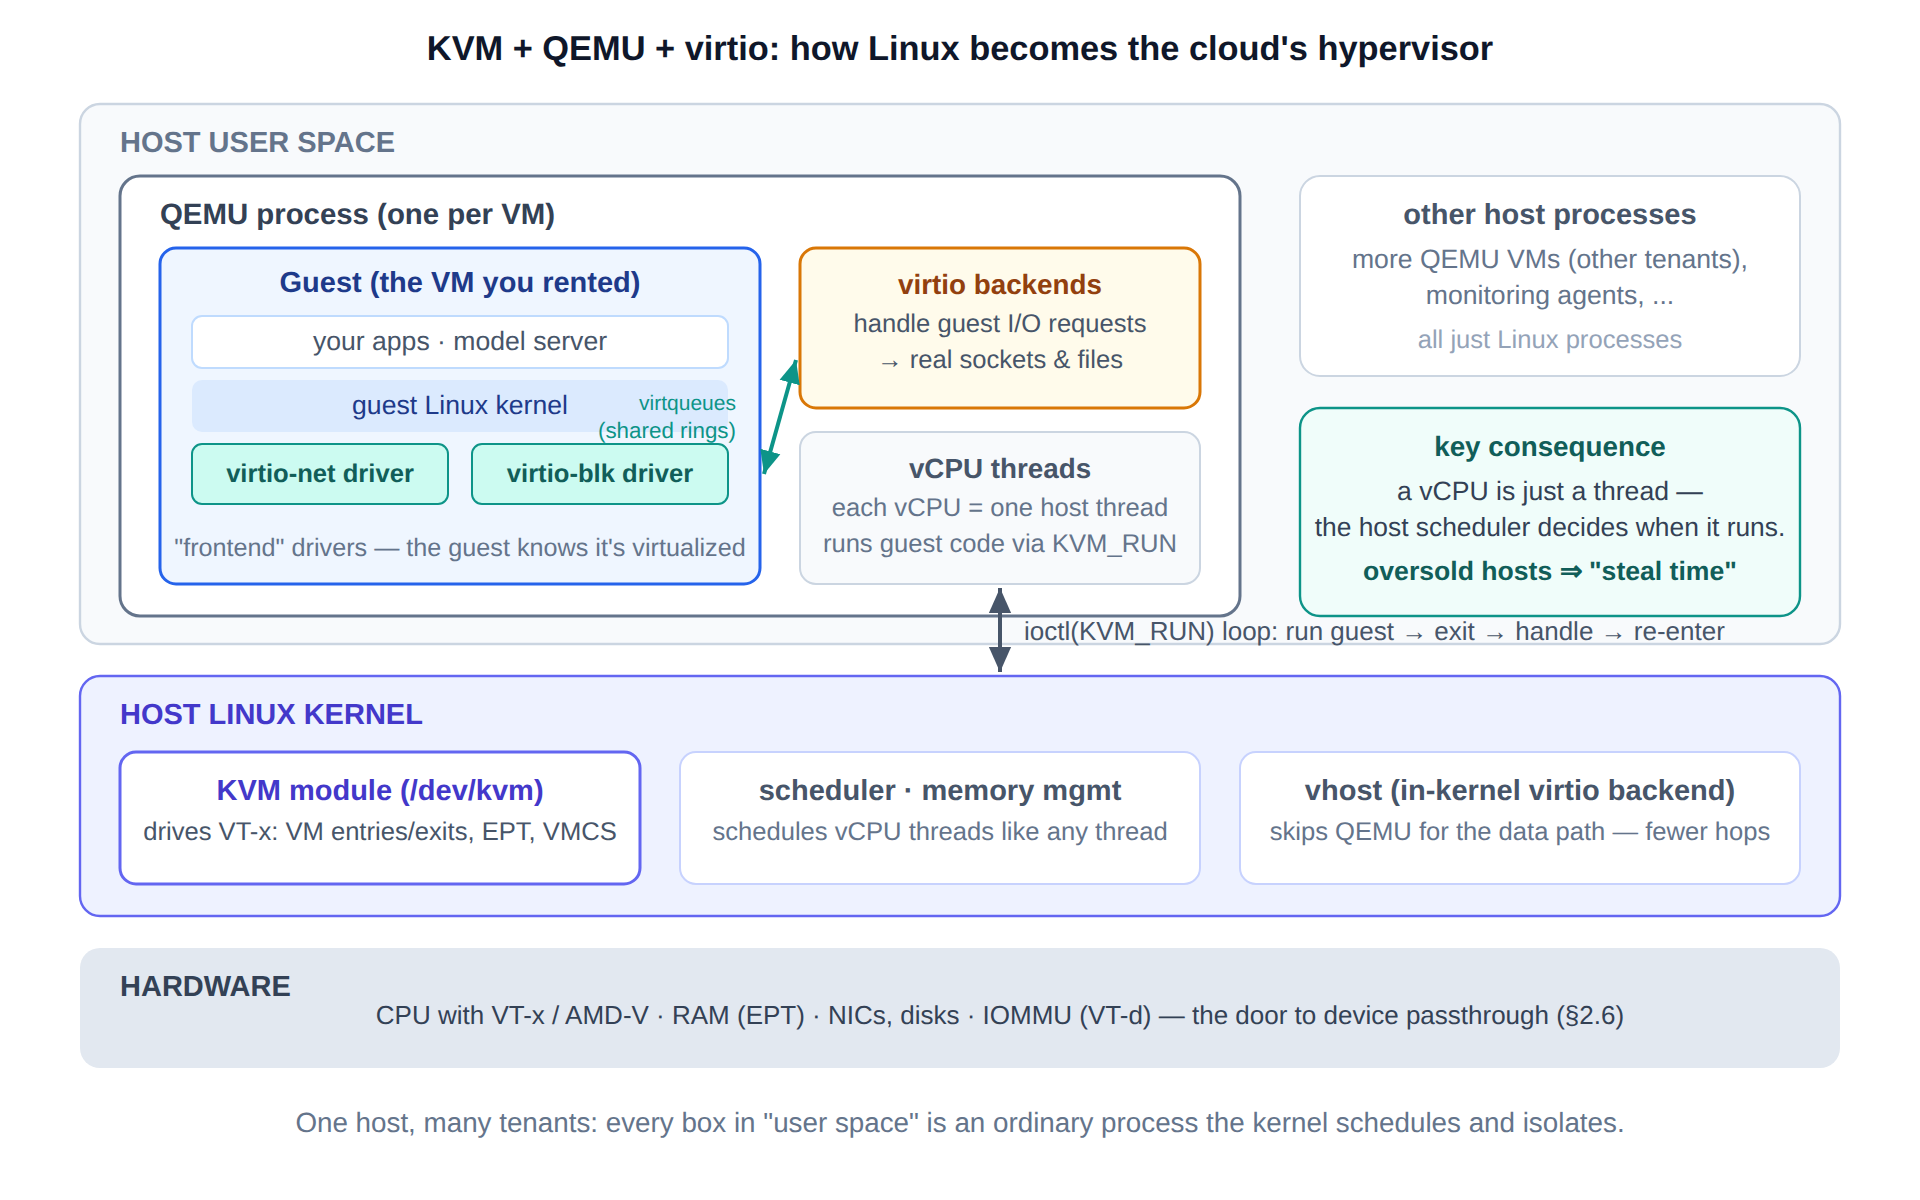
\includegraphics{figures/fig2-4_kvm_virtio.png}}\\[3pt]
  \figcaption{Figure 2-4  The KVM/QEMU/virtio stack. KVM (kernel) drives VT-x; QEMU (one userspace process per VM) provides devices; virtio replaces the illusion of hardware with an honest, fast interface. A vCPU is just a host thread.}
\end{tbbfigure}

\subsection*{The division of labor}

\begin{tbbitemize}
  \item \textbf{KVM (in the kernel)} exposes \code{/\allowbreak dev/\allowbreak kvm}, a small ioctl API: create a VM, give it memory, create vCPUs, and — the heart of it — \code{KVM\_RUN}. It programs the VMCS, executes VM entries, and fields VM exits, handling the hot, simple ones (EPT faults, most MSR accesses) right in the kernel.
  \item \textbf{QEMU (in userspace, one process per VM)} does everything else: it allocates the guest's memory (just process memory!), loads its firmware or kernel, and — its signature job — provides the \textbf{device model}: software impersonations of NICs, disks, serial ports, and the rest of a motherboard's population. When a VM exit is about device I/O, KVM hands it up to QEMU, whose device code figures out what the guest was trying to do to the "hardware" and does the real-world equivalent through ordinary Linux syscalls — a packet onto a real socket, a block written to a real file.
  \item \textbf{The host Linux kernel} supplies what neither reimplements: its scheduler runs vCPUs, its memory manager backs guest RAM, its drivers and filesystems carry the actual I/O.
\end{tbbitemize}

The run loop that animates a guest is worth seeing once in prose. A vCPU thread calls \code{ioctl(KVM\_RUN)}; the kernel VM-enters; the guest computes natively in non-root mode until something exits; KVM either handles the exit and re-enters immediately, or returns to QEMU for device work and then re-enters. Rinse, repeat, for the lifetime of the VM. Everything you learned in 2.3 — exit reasons, exit costs — is this loop's inner economics.

\subsection*{A vCPU is just a thread — and why your p99 should care}

Look again at where vCPUs live in Figure 2-4: they are \textbf{ordinary host threads}. Do not take the figure's word for it — on any Linux box running a KVM guest (your laptop with virt-manager will do), the host will show you:

\begin{terminalbox}
\begin{Verbatim}[breaklines=true,breakanywhere=true,fontsize=\small,formatcom=\color{tbbtermfg},codes=\tbbcodeactive]
# on the HOST, with one 4-vCPU guest running:
$ pstree -p $(pgrep -of qemu) | head -5
qemu-system-x86(9114)-+-{CPU 0/KVM}(9131)
                      |-{CPU 1/KVM}(9132)
                      |-{CPU 2/KVM}(9133)
                      |-{CPU 3/KVM}(9134)
$ ps -o pid,psr,pcpu,comm -Lp 9114 | grep CPU  # psr = core hosting it
 9131  3  99.2  CPU 0/KVM     # "processor 0" = thread 9131, on core 3
 9132 11   1.0  CPU 1/KVM     # idle vCPU, parked on core 11
# renice it, pin it, cgroup it - everything Linux does to threads applies.
\end{Verbatim}
\end{terminalbox}
\figcaption{Transcript 2-2  The guest's four "processors," seen from the host: four schedulable threads inside one QEMU process. Everything that follows — overcommit, steal time, dedicated cores — is ordinary thread scheduling wearing a costume.}

This one fact produces several cloud phenomena you will meet operationally:

\begin{tbbitemize}
  \item \textbf{Overcommit.} The host can create more vCPUs than physical cores, betting tenants won't peak together — the same economics as airline seats. Budget instance families are priced on this bet.
  \item \textbf{Steal time.} When the host scheduler runs \textit{someone else} during your vCPU's runnable time, your guest experiences time passing without cycles — visible as \code{\%st} in \code{top} inside the guest. For latency-sensitive serving, steal is pure tail-latency poison: a request that arrives during a stolen slice waits invisibly. This is why serious serving fleets buy instance types with dedicated cores, and why "my p99 spikes but my CPU graph looks fine" is a question whose answer may live one layer below your VM.
  \item \textbf{Noisy neighbors, bounded.} Schedulers and cgroup weights (Chapter 3!) bound how badly tenants can hurt each other — the referee from 2.1, implemented by the same kernel mechanisms you will manipulate next week.
\end{tbbitemize}

Steal time deserves its own exhibit, because it is the one virtualization artifact you are most likely to meet in production telemetry — and the easiest to misdiagnose as an application problem:

\begin{terminalbox}
\begin{Verbatim}[breaklines=true,breakanywhere=true,fontsize=\small,formatcom=\color{tbbtermfg},codes=\tbbcodeactive]
# inside a guest on a busy (oversold) host, during a load test:
$ top -bn1 | grep "%Cpu"
%Cpu(s): 41.2 us, 3.1 sy, 0.0 ni, 30.5 id, 0.2 wa, 0.0 hi, 0.6 si, 24.4 st
#                                                                  ^^^^^^^
# st = steal: 24.4% of this guest's runnable time went to... someone else.
# no process inside the guest will ever show this in its profile.
$ grep -A1 steal /proc/stat | head -2      # the raw counter, if you script it
cpu  184023 340 44522 830112 902 0 4211 267001 0 0
#                                        ^^^^^^ jiffies stolen since boot
\end{Verbatim}
\end{terminalbox}
\figcaption{Transcript 2-3  Steal time, caught in the act. The guest was runnable; the host scheduler ran another tenant; your request waited a slice it cannot see. p99 spikes with a clean CPU graph — one layer down is where the answer lives.}

\subsection*{The device problem, and virtio's honest answer}

Now the third pillar of virtualization: I/O. The full-illusion approach is \textbf{device emulation}: QEMU impersonates a specific, venerable real NIC (the Intel e1000 is the classic), and the guest runs its stock driver. Equivalence is perfect — any OS with an e1000 driver just works — but consider the price. That driver was written for hardware where a register write costs nanoseconds; against an emulated device \textbf{every register access is a VM exit} into userspace. Sending one packet touches the device many times: exit, exit, exit. Emulated I/O can be an order of magnitude or more slower than native, drowning in world switches.

The fix is Section 2.2's paravirtual idea, reborn where it works best. \textbf{virtio} (Rusty Russell, 2008 — now a standard) says: stop pretending. Present the guest a device that is \textit{openly virtual}, with an interface designed for the actual situation — two software components passing buffers through shared memory. The guest loads a \textbf{frontend driver} (\code{virtio-net}, \code{virtio-blk}, ...); the hypervisor side runs the matching \textbf{backend}; between them sit \textbf{virtqueues} — ring buffers in guest memory where the guest posts batches of buffer descriptors and the backend consumes them. The guest "kicks" the backend with a single lightweight exit \textit{per batch} (not per register), completions come back via interrupt or are picked up during polling, and under load the rings stay busy with almost no exits at all. Same physics as dynamic batching in Week 10, one layer down: \textbf{amortize the expensive crossing over many units of work.}

Two refinements complete the picture. \textbf{vhost} moves the backend from QEMU into the host kernel, cutting the userspace hop for the data path (and vhost-user moves it instead into a dedicated userspace switch, as DPDK-based network stacks do). And for the highest tier, hardware re-enters: \textbf{SR-IOV} lets one physical NIC present many lightweight \textit{virtual functions}, each safely assignable straight into a guest via the IOMMU — device "emulation" done by the silicon itself. Hold that thought: assigning real hardware into a guest is exactly how GPUs will reach your VM in Section 2.6.

\begin{calloutbox}{tbbteal}{tbbtealfill}
{\normalsize\bfseries\color{tbbx115E59}Box 2-2  AWS Nitro: driving the virtualization tax toward zero}\par\vspace{3pt}
Follow the logic of this section to its end and you arrive at Nitro, the system under modern EC2. AWS moved the device models \textit{out of software entirely} — networking, storage, and management run on dedicated \textbf{Nitro cards} (custom silicon), presented to guests as directly-assigned hardware. What remains on the host CPU is a deliberately minimal, KVM-based hypervisor with no QEMU in the data path. Guests get near-bare-metal performance; the host burns almost no cores on plumbing; and the same architecture yields true bare-metal instances (the Nitro cards \textit{are} the motherboard's I/O). The historical arc is tidy: EC2 began on paravirtualized Xen (2006), and two decades of exit-elimination ended with the exits' work moved into hardware (2017–).
\end{calloutbox}

\vspace{3.0pt}

\begin{calloutbox}{tbbpurple}{tbbpurplefill}
{\normalsize\bfseries\color{tbbpurple}Think About It}\par\vspace{3pt}
\begin{tbbitemize}
  \item Trace one HTTPS response from your model server in a guest, out to a client: which components from Figure 2-4 does each byte cross with (a) emulated e1000, (b) virtio + vhost, (c) SR-IOV? Count the world switches qualitatively.
  \item Inside a guest, \code{top} shows 25\% steal during your load test's latency spikes. What are your options, short of changing cloud providers? (Consider instance families, and what "dedicated" costs.)
\end{tbbitemize}
\end{calloutbox}

\section{How Small Can a VM Get? MicroVMs and the Isolation Spectrum}

Everything so far assumed the classic cloud unit: a rented server that lives for hours to years. The 2010s added a new extreme — serverless functions and per-request sandboxes that live for \textbf{milliseconds to minutes}, belong to \textbf{mutually distrusting strangers}, and must be packed \textbf{thousands to a host} to make economic sense. At that scale the classic VM is the wrong shape: you cannot bill in 100 ms units if creating the environment takes 40 s and 500 MB. The industry's response reshaped virtualization itself, and the way to understand it is as a spectrum (Figure 2-5): \textit{what stands between tenant code and the host kernel, and what does each layer cost?}

\begin{tbbfigure}
  \adjustbox{max width=0.94\linewidth,max totalheight=0.46\textheight}{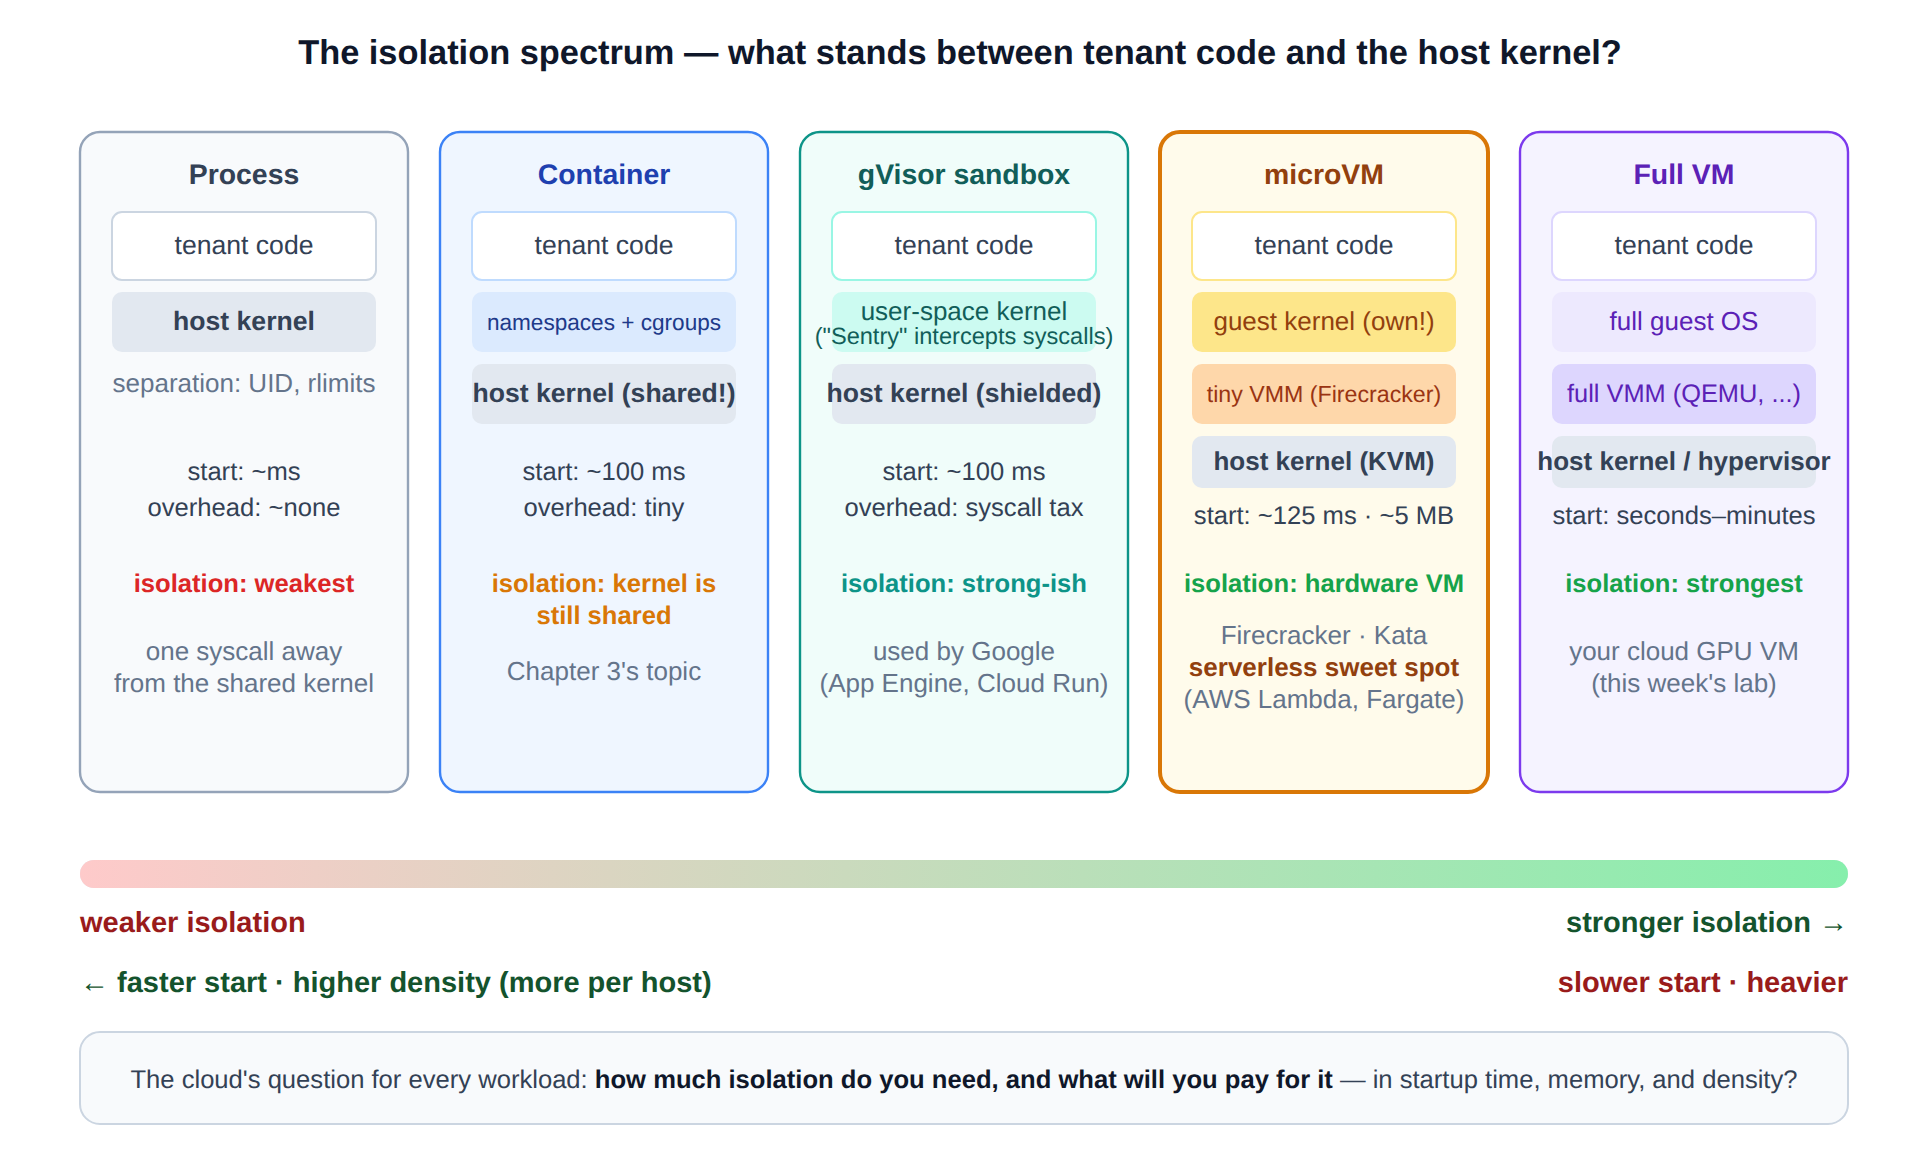
\includegraphics{figures/fig2-5_spectrum.png}}\\[3pt]
  \figcaption{Figure 2-5  The isolation spectrum. Rightward: more layers between tenant and host kernel, stronger isolation, slower start, lower density. The serverless sweet spot is the microVM.}
\end{tbbfigure}

\subsection*{Why containers alone don't settle it}

Next week you will build containers from kernel primitives, so here we need only the security-relevant silhouette: a container is a group of ordinary processes given a private \textit{view} (namespaces) and bounded \textit{share} (cgroups) — \textbf{of a kernel it still shares with everyone else on the host.} Startup is \textasciitilde{}100 ms and overhead is near zero, which is why containers won the packaging war. But the isolation boundary is the syscall interface: hundreds of entry points into one kernel whose single vulnerability is every tenant's vulnerability. Container escapes are not hypothetical; they are a recurring genre of CVE. For \textit{your own} workloads sharing \textit{your} cluster, that risk is usually acceptable and Kubernetes is built on exactly that judgment. For running \textbf{arbitrary strangers' code} — a public FaaS, a CI service, an AI-agent sandbox executing model-generated programs — most operators judge a shared kernel insufficient. (That last example is very much of this course's era: "run the code the LLM just wrote" is a multi-tenant isolation problem par excellence.)

\subsection*{Three answers between container and VM}

\textbf{gVisor (Google, 2018)} keeps the container shape but inserts a bodyguard: the \textit{Sentry}, a user-space kernel written in Go, intercepts the application's syscalls and services them itself, touching the real host kernel through a drastically narrowed, hardened set of calls. Tenant code thus never speaks to the host kernel directly — a kernel exploit must first pierce a second, memory-safe kernel. The price is a syscall tax (heavy I/O workloads feel it) and imperfect compatibility at the edges of Linux behavior. Google runs vast fleets on it (App Engine, Cloud Run, Cloud Functions).

\textbf{Kata Containers} takes the other direction: keep the container \textit{interface}, change the \textit{implementation} to a real hardware VM — each pod gets its own guest kernel inside a lightweight VM, slotting into Kubernetes via the standard runtime plumbing (Chapter 4). You buy VM-grade isolation for container-shaped workflows, at the cost of VM-shaped overhead per pod — mitigated by pairing Kata with a minimal VMM underneath, which brings us to the star of this section.

\textbf{Firecracker (AWS, open-sourced 2018; NSDI 2020)} answers a brutally specific question: what is the \textit{minimum} virtual machine that Lambda actually needs? The answer (Figure 2-6): a VMM that keeps KVM and hardware isolation but deletes the general-purpose device museum. No BIOS — the guest kernel is loaded directly. No PCI enumeration. No VGA, USB, sound; no live migration. Just virtio-net, virtio-block, a vsock channel, a serial console, and a REST API to drive it — \textasciitilde{}50 k lines of Rust (vs. QEMU's millions of C), each microVM further caged by a seccomp-restricted "jailer." The published numbers rewired the industry's intuition for what a VM costs: \textbf{boot to guest userspace in under 125 ms, under 5 MB of VMM overhead per microVM, 150 microVMs creatable per second per host} — a VM that behaves, operationally, like a process. This is what actually runs every AWS Lambda invocation and Fargate task, at millions-per-second scale.

\begin{tbbfigure}
  \adjustbox{max width=0.94\linewidth,max totalheight=0.46\textheight}{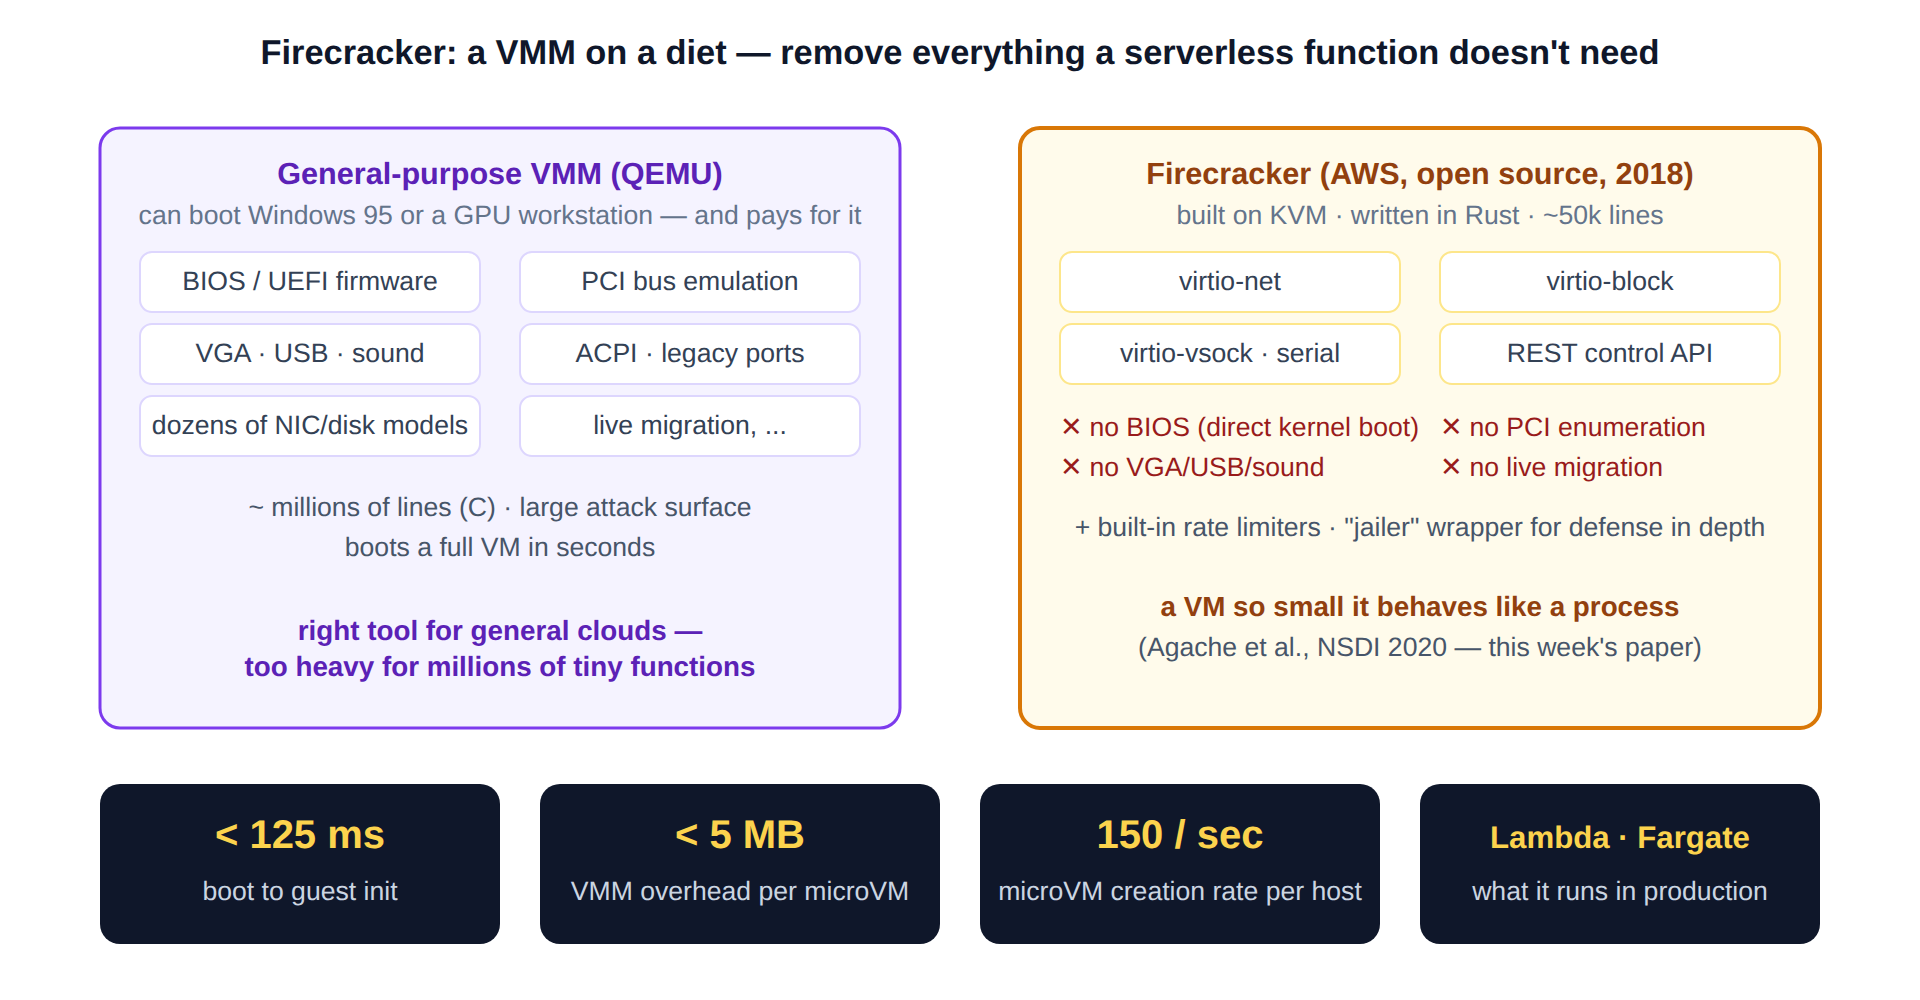
\includegraphics{figures/fig2-6_firecracker.png}}\\[3pt]
  \figcaption{Figure 2-6  Firecracker: keep KVM, delete the device museum. The numbers — 125 ms, 5 MB, 150/s — are from the NSDI 2020 paper, this week's required reading.}
\end{tbbfigure}

\begin{tbbtablewrap}
  \begin{tabular}{@{}>{\raggedright\arraybackslash}m{\dimexpr 0.2021\tbltextwidth-2\tabcolsep\relax} >{\raggedright\arraybackslash}m{\dimexpr 0.1968\tbltextwidth-2\tabcolsep\relax} >{\raggedright\arraybackslash}m{\dimexpr 0.1968\tbltextwidth-2\tabcolsep\relax} >{\raggedright\arraybackslash}m{\dimexpr 0.2021\tbltextwidth-2\tabcolsep\relax} >{\raggedright\arraybackslash}m{\dimexpr 0.2021\tbltextwidth-2\tabcolsep\relax}@{}}
  \arrayrulecolor{tbbnavy}\specialrule{1pt}{0pt}{0pt}
  \rowcolor{tbbtablehead}{\centering \bfseries\color{tbbnavy} } & {\centering \bfseries\color{tbbnavy}Container} & {\centering \bfseries\color{tbbnavy}gVisor} & {\centering \bfseries\color{tbbnavy}microVM (FC/Kata)} & {\centering \bfseries\color{tbbnavy}Full VM} \\
  \arrayrulecolor{tbbnavy}\specialrule{0.7pt}{0pt}{2pt}
  {\textbf{Kernel}} & {host's, shared} & {user-space proxy kernel} & {own guest kernel} & {own guest kernel} \\
  \arrayrulecolor{tbbtableborder}\hline
  {\textbf{Isolation boundary}} & {syscall interface} & {Sentry + narrowed syscalls} & {hardware (VT-x)} & {hardware (VT-x)} \\
  \arrayrulecolor{tbbtableborder}\hline
  {\textbf{Startup}} & {\textasciitilde{}100 ms} & {\textasciitilde{}100 ms} & {\textasciitilde{}125 ms–1 s} & {seconds–minutes} \\
  \arrayrulecolor{tbbtableborder}\hline
  {\textbf{Per-instance overhead}} & {≈ 0} & {syscall tax} & {\textasciitilde{}5 MB + guest kernel} & {100s of MB} \\
  \arrayrulecolor{tbbtableborder}\hline
  {\textbf{Typical use}} & {your own workloads; K8s default} & {multi-tenant PaaS (Google)} & {FaaS; untrusted code (AWS)} & {rented cloud servers} \\
  \arrayrulecolor{tbbnavy}\specialrule{1pt}{2pt}{0pt}
  \end{tabular}\par
  \figcaption{Table 2-2  Isolation options compared (orders of magnitude, not benchmarks)}
\end{tbbtablewrap}

\subsection*{What this means for serving (the Week 12 thread)}

Connect this to Chapter 1's scale-to-zero story and the picture sharpens usefully. Firecracker proves the \textit{environment} can appear in \textasciitilde{}125 ms — so when a GPU-backed model endpoint cold-starts in 30–60 s, the microVM is not the culprit. The time went to scheduling a GPU host, pulling a multi-gigabyte container image, loading tens of gigabytes of weights into GPU memory, and warming runtime caches. That decomposition \textit{is} the Week 12 lesson in embryo: virtualization has done its part; the remaining cold-start engineering is about images, weights, and GPU state — which is why techniques like snapshot/restore of a \textit{loaded} VM (Firecracker snapshots are one thread of current serverless-GPU research and practice) are where the frontier lies. When a serverless GPU platform quotes you a cold start, you now know how to audit the number.

\begin{calloutbox}{tbbpurple}{tbbpurplefill}
{\normalsize\bfseries\color{tbbpurple}Think About It}\par\vspace{3pt}
\begin{tbbitemize}
  \item Your team will run untrusted, model-generated Python for an AI-agent product. Argue container vs. gVisor vs. Firecracker for this sandbox along: blast radius of a kernel 0-day, startup latency budget (interactive!), density per host, and GPU access (peek at 2.6).
  \item Density math: a host has 384 GB RAM for tenants. Estimate how many idle 128 MB-heap functions fit as (a) containers (\textasciitilde{}0 overhead), (b) Firecracker microVMs (+5 MB + \textasciitilde{}20 MB guest kernel each), (c) full VMs (+300 MB each). What does the answer do to per-invocation pricing?
\end{tbbitemize}
\end{calloutbox}

\section{GPUs in the Cloud: Instances, Passthrough, and Sharing}

Everything in this chapter so far virtualized the CPU, memory, and I/O. Now add the component this course actually revolves around — and notice that the GPU stubbornly resists the whole playbook. There is no "VT-x for GPUs": no architectural non-root mode, no hardware trap-and-emulate for CUDA. A GPU holds gigabytes of context that cannot be world-switched in a microsecond, is driven by an enormous proprietary driver stack, and was designed for one demanding owner, not polite time-sharing. So the cloud's answers for "how does a tenant get a GPU?" look different from everything above — and the three of them (Figure 2-7) will follow you to Week 12, because \textbf{how finely a GPU can be shared is a serving-economics question wearing a virtualization costume.}

\subsection*{First, the shapes on the price list: GPU instance families}

Providers package GPUs into instance families that mirror Chapter 1's training-vs-inference divide. \textbf{Training shapes} put 8 flagship accelerators (H100/H200/B200-class) in one chassis with NVLink among them and very fast fabric between chassis — AWS's P-family, GCP's A3, Azure's ND-series. \textbf{Inference shapes} attach one to a few smaller GPUs (T4, L4, A10-class) to modest CPU counts — AWS's G-family, GCP's G2 — at an order of magnitude lower hourly cost; this is where our lab lives (a T4 instance such as AWS g4dn or a GCP N1+T4 pairing). Two practical notes that surprise beginners: GPU instances are often \textbf{quota-gated} (you must request access before you can launch — do this early in the lab), and the GPU's spec sheet matters less than its \textbf{VRAM} for our purposes, per Chapter 1's fits-in-memory arithmetic.

\begin{tbbtablewrap}
  \begin{tabular}{@{}>{\raggedright\arraybackslash}m{\dimexpr 0.1862\tbltextwidth-2\tabcolsep\relax} >{\raggedright\arraybackslash}m{\dimexpr 0.2660\tbltextwidth-2\tabcolsep\relax} >{\raggedright\arraybackslash}m{\dimexpr 0.1915\tbltextwidth-2\tabcolsep\relax} >{\raggedright\arraybackslash}m{\dimexpr 0.3564\tbltextwidth-2\tabcolsep\relax}@{}}
  \arrayrulecolor{tbbnavy}\specialrule{1pt}{0pt}{0pt}
  \rowcolor{tbbtablehead}{\centering \bfseries\color{tbbnavy}GPU (VRAM)} & {\centering \bfseries\color{tbbnavy}Typical instance} & {\centering \bfseries\color{tbbnavy}Rough \$/hr} & {\centering \bfseries\color{tbbnavy}Serving sweet spot} \\
  \arrayrulecolor{tbbnavy}\specialrule{0.7pt}{0pt}{2pt}
  {\textbf{T4 (16 GB)}} & {AWS g4dn.xlarge · GCP N1+T4} & {≈ \$0.5} & {This course's lab baseline; small models, INT8 inference} \\
  \arrayrulecolor{tbbtableborder}\hline
  {\textbf{L4 (24 GB)}} & {GCP g2-standard-4 · AWS g6} & {≈ \$0.7–1.0} & {The modern inference workhorse; low power per token} \\
  \arrayrulecolor{tbbtableborder}\hline
  {\textbf{A10G (24 GB)}} & {AWS g5.xlarge} & {≈ \$1.0} & {Mid-size models — Chapter 1's Exhibit 1-B rented exactly this} \\
  \arrayrulecolor{tbbtableborder}\hline
  {\textbf{A100 (80 GB)}} & {AWS p4d (÷8) · GCP a2} & {≈ \$3–5 per GPU} & {Big models (quantized 70B), MIG host for slicing (§ below)} \\
  \arrayrulecolor{tbbtableborder}\hline
  {\textbf{H100 (80 GB)}} & {AWS p5 (÷8) · GCP a3} & {\$2–7 per GPU (channel-dependent)} & {Frontier serving and training; NVLink-coupled} \\
  \arrayrulecolor{tbbtableborder}\hline
  {\textcolor{tbbgray}{(ref) B200 (192 GB)}} & {\textcolor{tbbgray}{next generation}} & {\textcolor{tbbgray}{\$4–6+}} & {\textcolor{tbbgray}{raises the per-GPU ceiling again}} \\
  \arrayrulecolor{tbbnavy}\specialrule{1pt}{2pt}{0pt}
  \end{tabular}\par
  \figcaption{Table 2-3  The serving fleet, priced (illustrative on-demand figures, mid-2026 — the structure outlives the numbers)}
\end{tbbtablewrap}

Read the table with Chapter 1's two lenses and it becomes a decision tool rather than a catalog. \textbf{Binding dimension:} if your quantized model needs 11 GB, the T4 and everything above it all \textit{work} — but only the T4-to-L4 band works \textit{economically}; validating a model on T4 economics and then deploying it on an A100 "to be safe" pays 6–10× per hour for VRAM and FLOPs that never bind. \textbf{Utilization:} the price column is per hour whether you serve or idle, so the fleet question is never "which GPU is best?" but "which is the cheapest card that meets the SLO at the utilization I can actually sustain?" This table returns in Week 12 when autoscaling and GPU sharing turn it into an optimization problem — remember it as \textit{the fleet table}.

\subsection*{How a VM gets a whole GPU: PCIe passthrough}

\begin{terminalbox}
\begin{Verbatim}[breaklines=true,breakanywhere=true,fontsize=\small,formatcom=\color{tbbtermfg},codes=\tbbcodeactive]
# on this week's rented VM - recall Exhibit 2-A: everything so far was fake
$ lspci | grep -i nvidia
00:1e.0 3D controller: NVIDIA Corporation TU104GL [Tesla T4]
$ nvidia-smi --query-gpu=name,driver_version,memory.total --format=csv
name, driver_version, memory.total [MiB]
Tesla T4, 550.54.15, 16384 MiB
# a REAL PCI device, running the REAL driver, inside the fake machine.
# the one component the hypervisor did not fake. how? and why not?
\end{Verbatim}
\end{terminalbox}
\figcaption{Transcript 2-4  The exception in the illusion. The disk is virtio, the clock is kvm-clock, the CPU model is a menu choice — but the T4 is physical silicon, handed through. This subsection explains the how (VFIO + IOMMU) and the price (one tenant per card).}

When you launch that g4dn this week, the T4 your \code{nvidia-smi} shows is \textbf{the physical card} — not an emulation, not a proxy. The mechanism is \textbf{PCIe passthrough}: the host (via Linux's VFIO framework) detaches the device from itself and maps it into your guest, which loads the real NVIDIA driver and speaks to real silicon. The enabling hardware is the \textbf{IOMMU} (Intel VT-d / AMD-Vi) from Table 2-1: GPUs are DMA engines that read and write memory directly, and an unpoliced DMA engine handed to a tenant could read the whole host. The IOMMU gives the device its own address translation — DMA addresses go through hypervisor-controlled tables exactly as guest memory accesses go through EPT — so the GPU can only touch its own guest's pages. Passthrough is why cloud GPU performance is near-native (the data path involves no hypervisor at all after setup), and its limitation is equally structural: \textbf{the unit of allocation is one whole physical GPU.} One tenant, one card; nothing to referee. (It also pins the VM to the host — no live migration with a passed-through device — one reason GPU instances get interrupted for maintenance rather than moved.)

\subsection*{Sharing one GPU: time-slicing, vGPU, MPS — and MIG}

Whole-GPU allocation collides with Chapter 1's utilization problem the moment models are small: a 3 GB model on an 80 GB H100 wastes 96\% of the most expensive part in the rack. The sharing options differ in \textit{what enforces fairness} — software schedules, or silicon partitions (Figure 2-7).

\begin{tbbfigure}
  \adjustbox{max width=0.94\linewidth,max totalheight=0.46\textheight}{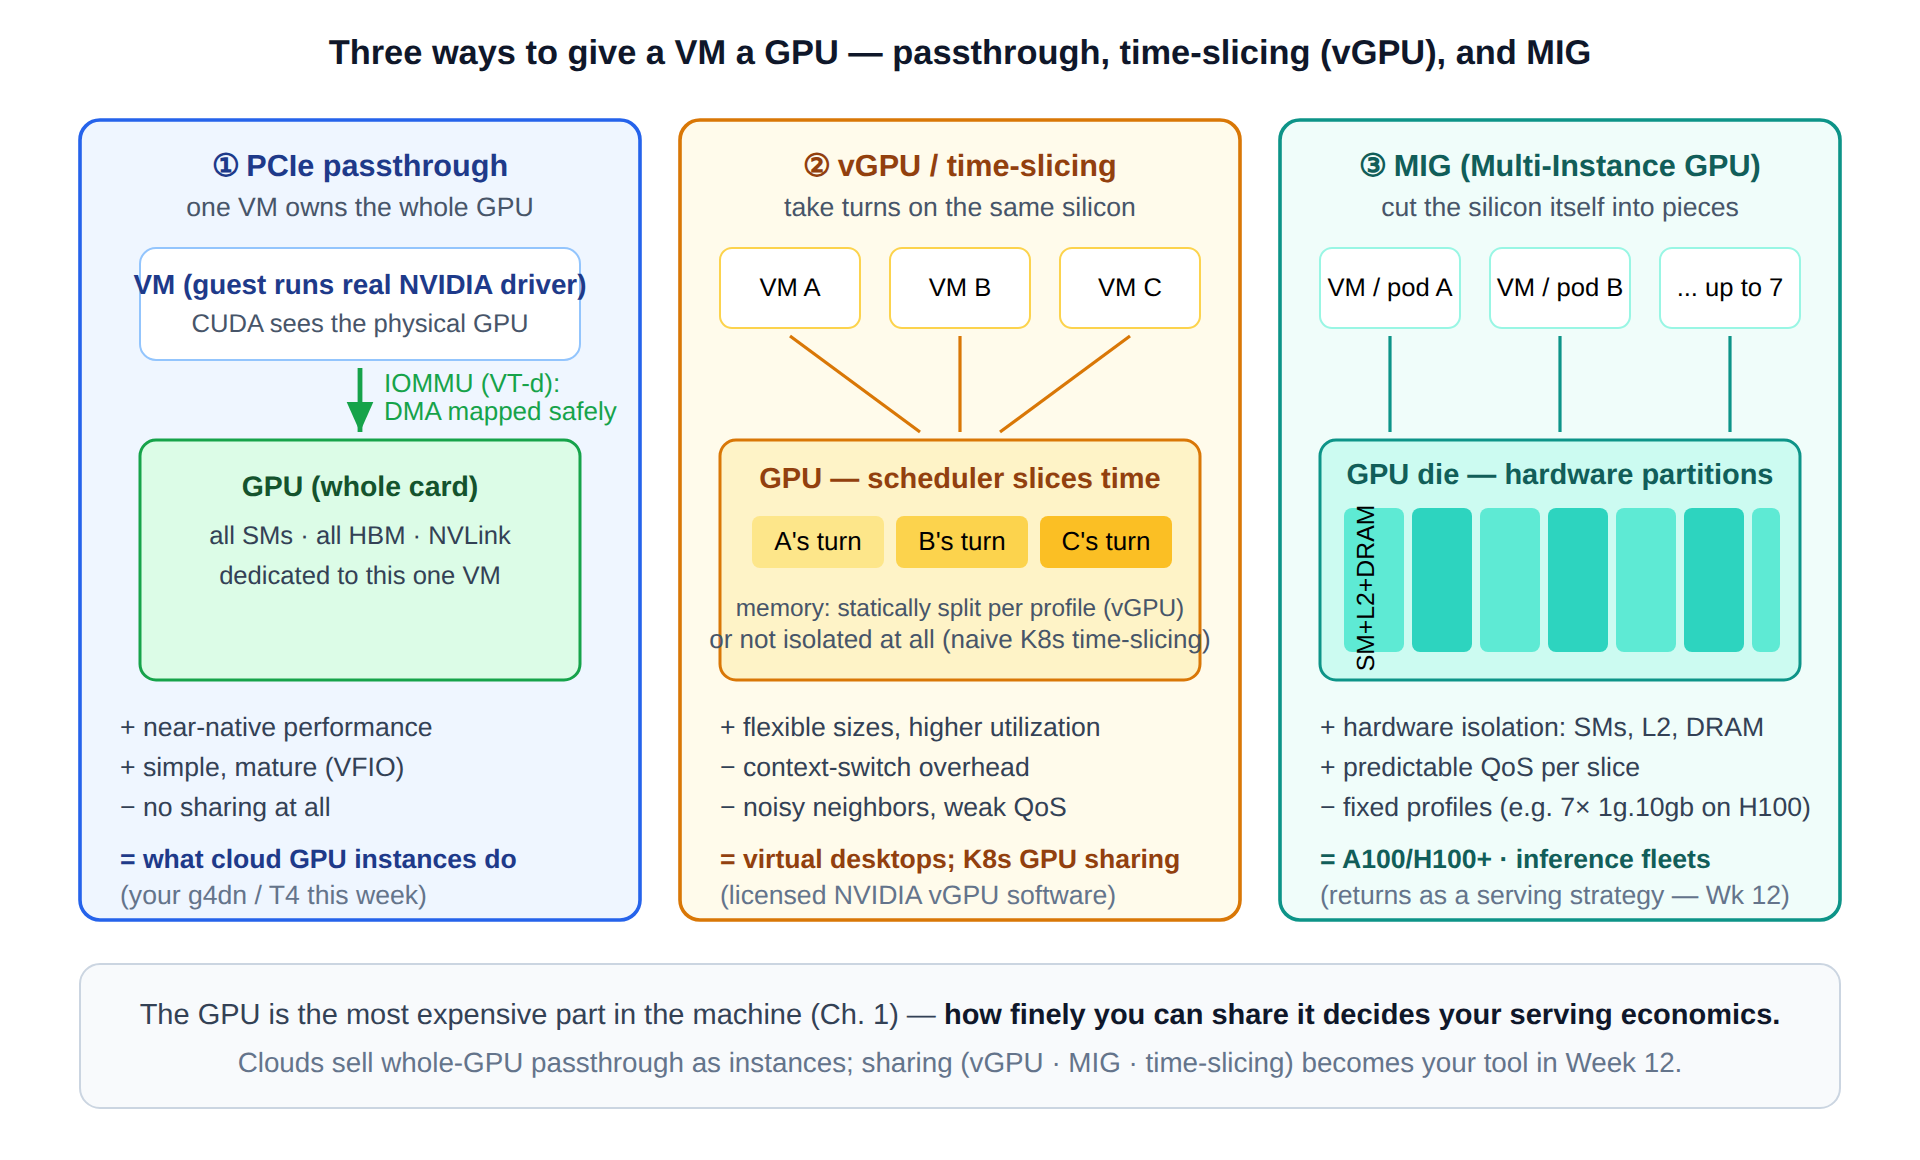
\includegraphics{figures/fig2-7_gpu_virt.png}}\\[3pt]
  \figcaption{Figure 2-7  Three ways to a GPU: exclusive passthrough (what instances sell), temporal sharing (vGPU/time-slicing/MPS), and spatial hardware partitioning (MIG).}
\end{tbbfigure}

\begin{tbbitemize}
  \item \textbf{Naive time-slicing} (as in Kubernetes' GPU time-slicing) lets multiple workloads take turns submitting to the same GPU. Nothing partitions memory and nothing guarantees turns are fair: one tenant can allocate all VRAM or hog long kernels. Acceptable among trusted, cooperative jobs; unfit for strangers or for tail-latency promises.
  \item \textbf{NVIDIA vGPU} productizes temporal sharing for VMs: licensed host software plus profiles that \textit{statically partition VRAM} (each vGPU owns its slice) while a scheduler time-slices compute among guests, each running near-normal drivers. Born for virtual desktops; workable for inference; compute QoS is still scheduler-grade, not hardware-grade.
  \item \textbf{MPS (Multi-Process Service)} shares at CUDA level \textit{within} one owner's processes — concurrent kernels from several processes on one GPU with optional resource caps. Excellent for co-locating your own models; provides no security boundary at all.
  \item \textbf{MIG (Multi-Instance GPU}, Ampere/A100 onward\textbf{)} finally does what the CPU did in 2005: moves isolation into the silicon. The die is partitioned into up to \textbf{seven instances}, each owning its own SM slice, L2 slice, and DRAM controllers/capacity — e.g., seven 1g.10gb instances from one H100-80GB, or mixed sizes like 3g.40gb + 2g.20gb + 2g.20gb. Each instance has hardware-enforced memory bandwidth and capacity, so a neighbor's tantrum cannot move your latency: \textbf{predictable p99 per slice}, the property serving fleets crave. The trade: fixed profile menu, instances don't cooperate on one job, and reconfiguring is disruptive — a rigidity-for-guarantees trade you will price out in Week 12.
\end{tbbitemize}

\begin{tbbtablewrap}
  \begin{tabular}{@{}>{\raggedright\arraybackslash}m{\dimexpr 0.2181\tbltextwidth-2\tabcolsep\relax} >{\raggedright\arraybackslash}m{\dimexpr 0.1915\tbltextwidth-2\tabcolsep\relax} >{\raggedright\arraybackslash}m{\dimexpr 0.1862\tbltextwidth-2\tabcolsep\relax} >{\raggedright\arraybackslash}m{\dimexpr 0.1809\tbltextwidth-2\tabcolsep\relax} >{\raggedright\arraybackslash}m{\dimexpr 0.2234\tbltextwidth-2\tabcolsep\relax}@{}}
  \arrayrulecolor{tbbnavy}\specialrule{1pt}{0pt}{0pt}
  \rowcolor{tbbtablehead}{\centering \bfseries\color{tbbnavy} } & {\centering \bfseries\color{tbbnavy}Time-slicing (K8s)} & {\centering \bfseries\color{tbbnavy}NVIDIA vGPU} & {\centering \bfseries\color{tbbnavy}MPS} & {\centering \bfseries\color{tbbnavy}MIG} \\
  \arrayrulecolor{tbbnavy}\specialrule{0.7pt}{0pt}{2pt}
  {\textbf{Sharing type}} & {temporal} & {temporal + static VRAM} & {concurrent (CUDA)} & {spatial (hardware)} \\
  \arrayrulecolor{tbbtableborder}\hline
  {\textbf{Memory isolation}} & {none} & {static partitions} & {none} & {hardware-enforced} \\
  \arrayrulecolor{tbbtableborder}\hline
  {\textbf{QoS / p99}} & {none} & {scheduler-grade} & {caps, no boundary} & {hardware-grade} \\
  \arrayrulecolor{tbbtableborder}\hline
  {\textbf{Security boundary}} & {no} & {VM-grade (licensed)} & {no} & {yes (per instance)} \\
  \arrayrulecolor{tbbtableborder}\hline
  {\textbf{Best for}} & {trusted batch jobs} & {VDI; mixed VMs} & {your own co-located models} & {multi-tenant inference} \\
  \arrayrulecolor{tbbnavy}\specialrule{1pt}{2pt}{0pt}
  \end{tabular}\par
  \figcaption{Table 2-4  GPU sharing options at a glance}
\end{tbbtablewrap}

One closing connection: notice that the GPU recapitulated the CPU's whole history in this chapter — exclusive ownership (like pre-virtualization servers), then software time-sharing with weak guarantees (like binary translation's era), then hardware-enforced partitions (MIG as the GPU's VT-x moment). Architecture rhymes.

\begin{calloutbox}{tbbpurple}{tbbpurplefill}
{\normalsize\bfseries\color{tbbpurple}Think About It}\par\vspace{3pt}
\begin{tbbitemize}
  \item Three internal inference services each need \textasciitilde{}15 GB VRAM and a p99 SLO. You have one H100-80GB. Argue MIG profile choice vs. MPS vs. three separate L4 instances — on isolation, utilization, cost, and failure blast radius.
  \item Why does passthrough prevent live migration, while virtio devices don't? (Think about what state lives where in each case.)
\end{tbbitemize}
\end{calloutbox}

\section{Lab: Your First Cloud GPU — Safely}

The lab makes the chapter concrete: you will create your cloud account, put \textbf{billing guardrails in place before anything else}, launch a GPU VM, meet the hardware through \code{nvidia-smi}, race CPU against GPU on the same inference job, and shut everything down without leaving a meter running. The detailed click-by-click lives in the lab handout (consoles change faster than textbooks); what belongs here is the \textit{why} behind each step and the numbers you should expect. Deliverable: a one-page report — your measured latencies, and three observations connecting them to this chapter.

\subsection*{Step 0 — money guardrails, before any compute}

Chapter 1 closed with "hourly billing = idle time is money"; this is where it becomes muscle memory. Before launching anything: \textbf{(a)} create a budget with alert thresholds (e.g., email at 50/80/100\% of \$10) in your provider's billing console; \textbf{(b)} confirm you are on educational credits and know where the meter reading lives; \textbf{(c)} internalize the two clocks — \textit{stopped} instances stop billing compute but \textbf{keep billing attached disk storage}, while \textit{terminated} instances release everything (and their disks, unless told otherwise). The classic beginner's bill is not the GPU-hour; it is the forgotten 200 GB volume attached to a long-stopped instance, or the instance that was "stopped" only in an abandoned browser tab. The lab checklist ends with the console showing \textbf{zero running instances and zero unattached volumes} — screenshot it for your report.

\subsection*{Steps 1–3 — quota, launch, meet the GPU}

Request GPU quota early (approval can take hours), pick the cheapest T4 shape in a nearby region (AWS \code{g4dn.xlarge} or GCP N1 + T4 class — a dollar-ish per hour, and Colab remains the no-account fallback for the measurement itself), choose a deep-learning OS image so drivers come preinstalled, and ssh in. Then read \code{nvidia-smi} like a systems person, because every field echoes this chapter: the \textbf{driver/CUDA versions} belong to the \textit{guest} — your VM runs the real driver because the T4 is \textbf{passed through} (§2.6); the \textbf{memory readout (0/16384 MiB)} is the VRAM budget that Chapter 1's arithmetic and Week 10's quantization manage; \textbf{utilization and the process list} are the metrics your Week 12 autoscaler and Week 14 dashboards will consume. Also run \code{lspci | grep -i nvidia} — the GPU sits on the guest's PCI bus like any physical card, which is passthrough made visible. And notice what your 40-second launch \textit{was}, mechanically: a control plane chose a host, a hypervisor (this chapter) materialized a guest, firmware-less or firmware-quick boot brought up a kernel, cloud-init personalized it. You have now watched a cold start with your own eyes; Week 12 industrializes the observation.

\subsection*{Step 4 — the measurement: CPU vs. GPU inference}

Run the handout's benchmark script: a small transformer (DistilBERT-class) or small CNN, same batch of inputs, timed on CPU then on GPU (PyTorch: the difference is one \code{.to("cuda")}). Protocol matters more than code: \textbf{warm up first} — the very first GPU call pays one-time costs (CUDA context, memory pools, kernel selection) and can be \textit{slower than CPU}; report it separately as your first personal cold-start datum, then time steady-state over \textasciitilde{}100 iterations. Sweep batch sizes (1, 8, 32, 64) and record both \textbf{per-batch latency and throughput}. Expected shape of results, order-of-magnitude: CPU tens of ms for batch-1 and scaling roughly linearly with batch; GPU a few ms at batch-1 and \textit{barely moving} as batch grows — until GPU throughput is 10–50× CPU's at batch 32–64. If GPU batch-1 underwhelms, you have rediscovered why: launch overhead and the PCIe hop dominate tiny work; parallel hardware pays when you feed it width. You have just measured, personally, Chapter 1's throughput-vs-latency tension and the entire motivation for Week 10's batching — which is precisely the kind of observation your report should make.

\begin{calloutbox}{tbbpurple}{tbbpurplefill}
{\normalsize\bfseries\color{tbbpurple}Lab checklist (the version that keeps your credits)}\par\vspace{3pt}
\begin{tbbitemize}
  \item Budget + alerts exist \textbf{before} first launch; you know the billing page.
  \item GPU quota requested early; cheapest T4 shape; nearby region; DL image (drivers included).
  \item \code{nvidia-smi} and \code{lspci} outputs saved; warm-up vs. steady-state timed separately; batch sweep recorded (1/8/32/64).
  \item Instance \textbf{terminated} (not just stopped) unless you have a reason; volumes checked; final console screenshot: nothing running, nothing orphaned.
  \item Report: numbers + three observations tying them to §2.3–§2.6 (e.g., steal time seen? warm-up cost? batch effect?).
\end{tbbitemize}
\end{calloutbox}

\vspace{3.0pt}

\begin{calloutbox}{tbbpurple}{tbbpurplefill}
{\normalsize\bfseries\color{tbbpurple}Think About It}\par\vspace{3pt}
\begin{tbbitemize}
  \item Your batch-1 GPU latency barely beats CPU, but batch-64 GPU throughput is 40× CPU. Your production traffic arrives one request at a time. What are your options? (You have just reinvented the agenda of Weeks 10–12.)
  \item Estimate: at \$0.53/hr for a g4dn.xlarge, what does your whole lab cost if you work efficiently for 2 hours? What does it cost if you forget the instance for a month? Which number do the guardrails target?
\end{tbbitemize}
\end{calloutbox}

\namedsection{Summary}{The Chapter in Twelve Points}

\qitem{1}{\textbf{The machine you rent doesn't exist — and it will tell you so.} A hypervisor (VMM) multiplexes one physical host into many isolated virtual machines, and the guest can read the confession itself (Exhibit 2-A): DMI strings naming a retailer, \code{systemd-detect-virt} answering \code{kvm}, even the clock arriving as \code{kvm-clock}. The software illusion is the foundation of per-hour billing, multi-tenancy, and elasticity.}

\qitem{2}{\textbf{Virtualization is a sixty-year-old answer to one question: expensive hardware, idle.} Act one: million-dollar mainframes → time-sharing and CP-67's per-user virtual machines (1967). Act two: the 2000s' server sprawl at 5–15\% utilization → VMware's consolidation. Act three: EC2's \$0.10 \textit{hour} (2006) — allocation became software, so compute got a meter. The GPU is living act one again; §2.6 is its acts two and three, in progress.}

\qitem{3}{\textbf{Popek \& Goldberg (1974)} defined the contract — equivalence, efficiency, resource control — and the theorem: trap-and-emulate works iff every sensitive instruction is privileged (i.e., traps). Classic x86 broke this with 17 sensitive-but-unprivileged instructions.}

\qitem{4}{Two software eras bridged the gap: \textbf{binary translation} (VMware — rewrite the guest on the fly; full virtualization for unmodified guests) and \textbf{paravirtualization} (Xen — modify the guest to make hypercalls; faster, needs source). The cooperating-guest idea survives today as virtio.}

\qitem{5}{\textbf{VT-x/AMD-V (2005–06)} added VMX root/non-root modes with the VMCS as the contract: the guest kernel runs in ring 0 again, dangerous operations cause hardware VM exits. \textbf{Exits are the currency of virtualization performance} — count them, cheapen them.}

\qitem{6}{\textbf{EPT/NPT} ended shadow page tables: two hardware-walked translations (guest VA → guest PA → host PA). Costs surface as heavier TLB misses — huge pages matter, especially for memory-hungry inference.}

\qitem{7}{\textbf{KVM + QEMU + virtio} is Linux as hypervisor: KVM drives VT-x from the kernel, QEMU provides the device model per-VM, virtio replaces device illusions with honest shared-memory virtqueues that batch work per exit. \textbf{A vCPU is just a host thread} — hence overcommit, steal time, and their tail-latency consequences.}

\qitem{8}{The \textbf{isolation spectrum} orders the options by what separates tenant code from the host kernel: process < container (shared kernel!) < gVisor (user-space kernel) < microVM < full VM — trading startup time and density against isolation strength.}

\qitem{9}{\textbf{Firecracker} is the serverless-era answer: keep KVM, delete the device museum. <125 ms boot, <5 MB overhead, 150 microVMs/s per host — a VM that behaves like a process; runs Lambda and Fargate. Its lesson for Week 12: the environment is no longer the cold-start bottleneck; images, weights, and GPU state are.}

\qitem{10}{\textbf{GPUs resist classic virtualization} — no VT-x equivalent — so clouds sell whole-card \textbf{PCIe passthrough} (via IOMMU/VFIO, near-native, no sharing; Transcript 2-4's "real card in a fake machine"), while sharing comes from \textbf{time-slicing/vGPU} (software fairness), \textbf{MPS} (co-located own workloads), or \textbf{MIG} (hardware partitions: up to 7 isolated instances with per-slice memory and predictable p99 — the GPU's VT-x moment).}

\qitem{11}{\textbf{The fleet table (Table 2-3) is a decision tool:} T4/L4/A10G for inference at \textasciitilde{}\$0.5–1.0/hr up to A100/H100 at several dollars per GPU — read it with Chapter 1's binding dimension (which card is the \textit{cheapest} that fits and meets the SLO?) and utilization lenses, never as a "bigger is safer" catalog.}

\qitem{12}{\textbf{Billing guardrails are an engineering practice:} budgets and alerts before first launch; stopped ≠ free (disks bill); terminated releases; the lab ends with an empty console — and with your first personally measured cold start and CPU-vs-GPU batching curve.}

\namedsection{Exercises}{}

\subsection*{A. Multiple choice}

\qitem{1}{Which of the following is NOT one of Popek \& Goldberg's requirements for a virtual machine monitor?}

\begin{tbboptions}
  \item ① Equivalence — guests behave as on real hardware
  \item ② Efficiency — most instructions run directly on the CPU
  \item ③ Resource control — the VMM fully controls physical resources
  \item ④ Portability — guests run unchanged on any CPU architecture
\end{tbboptions}

\qitem{2}{Under VT-x, what happens when a guest kernel running in VMX non-root mode executes an operation the hypervisor has configured as intervention-worthy (e.g., an I/O port access)?}

\begin{tbboptions}
  \item ① The instruction silently does nothing, as on classic x86
  \item ② The hardware performs a VM exit: guest state is saved to the VMCS and control transfers to the hypervisor in root mode
  \item ③ The guest kernel crashes with a privilege fault
  \item ④ The instruction is binary-translated on the fly
\end{tbboptions}

\qitem{3}{What problem do EPT/NPT solve?}

\begin{tbboptions}
  \item ① Translating guest-physical to host-physical addresses in hardware, eliminating software shadow page tables
  \item ② Encrypting guest memory against the hypervisor
  \item ③ Letting guests share page tables to save memory
  \item ④ Accelerating disk I/O through page-sized transfers
\end{tbboptions}

\qitem{4}{Why is a virtio device faster than an emulated e1000 NIC?}

\begin{tbboptions}
  \item ① virtio device code is written in a faster language
  \item ② virtio hardware is physically newer than e1000 hardware
  \item ③ The guest knowingly cooperates: work is batched through shared-memory virtqueues, costing \textasciitilde{}one exit per batch instead of a VM exit per register access
  \item ④ virtio bypasses the kernel entirely in all configurations
\end{tbboptions}

\qitem{5}{The key isolation difference between containers and (micro)VMs is:}

\begin{tbboptions}
  \item ① Containers cannot limit CPU or memory usage
  \item ② Containers on a host share the host's kernel, so the syscall interface is the security boundary; each VM brings its own kernel behind a hardware boundary
  \item ③ VMs cannot run Linux
  \item ④ There is no difference; the terms are interchangeable
\end{tbboptions}

\qitem{6}{Which GPU-sharing mechanism provides hardware-enforced memory and bandwidth isolation per tenant?}

\begin{tbboptions}
  \item ① Kubernetes time-slicing        ② NVIDIA MPS
  \item ③ MIG (Multi-Instance GPU)      ④ CUDA streams
\end{tbboptions}

\qitem{7}{A teammate argues: "Our EC2 instance must be a physical server — nvidia-smi shows a real Tesla T4 with the real NVIDIA driver." Which rebuttal is correct?}

\begin{tbboptions}
  \item ① They are right: a real GPU implies a real machine
  \item ② The GPU is emulated by QEMU like the disk and NIC, so it proves nothing
  \item ③ The machine is a KVM guest (dmidecode, systemd-detect-virt, kvm-clock all attest it); the T4 alone is physical, mapped in whole via PCIe passthrough — the one deliberate exception to the illusion
  \item ④ nvidia-smi cannot run inside virtual machines at all
\end{tbboptions}

\subsection*{B. Short answer}

\qitem{1}{Name the two CPU modes VT-x introduces, and state which one the hypervisor occupies.}

\qitem{2}{Your monitoring inside a guest shows high \code{\%st} (steal time) exactly during p99 latency spikes. In one sentence: what is physically happening, and name one remedy.}

\qitem{3}{Fill in the blanks: handing a physical GPU to a guest is called ( ㉠ ), and it is safe only because the ( ㉡ ) translates and polices the device's DMA.}

\qitem{4}{Firecracker boots a microVM in \textasciitilde{}125 ms, yet a serverless GPU model endpoint may cold-start in 30+ seconds. Name two places the remaining time goes.}

\qitem{5}{Your quantized model needs 11 GB of VRAM and meets its SLO on an L4 (\textasciitilde{}\$0.8/hr). A teammate proposes deploying on an A100-80GB (\textasciitilde{}\$4/hr) "to be safe." Name the two Chapter-1 lenses the fleet table applies against this, in one sentence each.}

\subsection*{C. Essay}

\qitem{1}{Explain why classic x86 was not virtualizable under Popek \& Goldberg's theorem, describe how binary translation and paravirtualization each worked around it (one strength and one cost each), and how VT-x resolved the problem architecturally.}

\qitem{2}{You are designing the sandbox for a public "AI agent" service that executes code written by an LLM on behalf of anonymous users. Choose a point on the isolation spectrum (container / gVisor / Firecracker microVM / full VM) and defend it against the two neighboring options, considering kernel blast radius, startup latency, per-host density, and operational complexity.}

\qitem{3}{Your team owns one H100-80GB and must serve three internal models (\textasciitilde{}15 GB VRAM each) with p99 SLOs, plus a nightly batch embedding job that would happily consume the whole card. Propose a GPU-sharing plan (any combination of MIG, MPS, time-slicing, scheduling by time of day), and justify it on isolation, utilization, and operational simplicity. State what you would measure to validate the plan.}

\namedsection{Answers and Commentary}{}

\subsection*{A. Multiple choice}

\qitem{1}{\textbf{④} The three requirements are equivalence, efficiency, and resource control. Portability across architectures is not among them — a VMM presents the \textit{same} architecture it runs on. (§2.2, Box 2-1)}

\qitem{2}{\textbf{②} That is precisely a VM exit: hardware saves guest state to the VMCS, records the exit reason, and enters root mode. ① was the \textit{pre}-VT-x pathology; ④ was VMware's software-era workaround. (§2.3)}

\qitem{3}{\textbf{①} EPT/NPT add a second, hypervisor-owned translation walked by the CPU, so guests manage their own page tables exit-free and shadow tables disappear. Costs move to TLB-miss latency — hence huge pages. (§2.3)}

\qitem{4}{\textbf{③} The e1000 illusion forces an exit per register touch; virtio's honest interface batches descriptors in shared rings with \textasciitilde{}one kick per batch. Cooperation beats illusion — paravirtualization's enduring lesson. (§2.4)}

\qitem{5}{\textbf{②} Containers isolate the \textit{view} and \textit{share} of one shared kernel (namespaces/cgroups — Chapter 3); VMs put a hardware boundary and a private kernel between tenant and host. This is the entire axis of Figure 2-5. (§2.5)}

\qitem{6}{\textbf{③} Only MIG partitions the silicon itself — SMs, L2, DRAM — giving hardware-grade QoS per instance. Time-slicing and MPS share temporally/concurrently without a hardware boundary. (§2.6)}

\qitem{7}{\textbf{③} Exhibit 2-A's evidence (DMI strings, \code{systemd-detect-virt}, \code{kvm-clock}) establishes the machine is virtual; Transcript 2-4 establishes the GPU is real anyway — passthrough via VFIO/IOMMU maps the physical card into the guest. A real device inside a virtual machine is the designed outcome, not a contradiction. (§2.1, §2.6)}

\subsection*{B. Short answer}

\qitem{1}{\textbf{VMX root mode} (hypervisor) and \textbf{VMX non-root mode} (guest). Both contain rings 0–3; the guest kernel gets its ring 0 back, under hardware supervision.}

\qitem{2}{The host scheduler is running other tenants' threads during your vCPU's runnable time — your "CPU" pauses invisibly. Remedies: dedicated-core instance types, fewer vCPUs per host (less overcommit), or moving latency-critical serving off shared families.}

\qitem{3}{㉠ \textbf{PCIe passthrough} (via VFIO); ㉡ \textbf{IOMMU} (Intel VT-d / AMD-Vi).}

\qitem{4}{Any two of: scheduling/finding a GPU host; pulling a multi-GB container image; loading tens of GB of model weights to GPU memory; CUDA/runtime initialization and cache warm-up. The microVM itself stopped being the bottleneck — that is Firecracker's achievement and Week 12's starting point.}

\qitem{5}{\textbf{Binding dimension:} the constraint is 11 GB of VRAM, which the L4's 24 GB already satisfies — the A100's extra 56 GB and FLOPs never bind, so they are pure cost. \textbf{Utilization/cost:} the meter runs per hour regardless; at \textasciitilde{}5× the price for the same delivered SLO, cost per request rises \textasciitilde{}5× while measured utilization of the paid-for card falls. "Safe" here means "safely wasteful."}

\subsection*{C. Essay (grading points)}

\qitem{1}{Full credit requires: the theorem (sensitive ⊆ privileged) and that 17 x86 instructions violated it, failing \textit{silently} (POPF is the canonical example); binary translation = rewrite guest kernel code on the fly, cache translations (strength: unmodified guests; cost: enormous complexity/edge cases); paravirtualization = modify guest source to hypercall (strength: speed, batching; cost: requires and forever maintains guest changes); VT-x = orthogonal root/non-root modes + VMCS, restoring ring 0 to the guest and making every sensitive operation reliably trap in hardware. Bonus for noting virtio as paravirtualization's descendant. (§2.2–2.3)}

\qitem{2}{A strong answer picks \textbf{Firecracker-style microVMs} and argues: hardware boundary against kernel 0-days (vs. container/gVisor whose ceiling is the shared kernel or a Go proxy), \textasciitilde{}125 ms boots within interactive budgets, \textasciitilde{}5 MB overhead keeps density in the thousands, and production precedent (Lambda). It should concede honestly: more moving parts than containers, a syscall-compat story simpler than gVisor's but device/GPU access harder than containers'. gVisor is a defensible alternative if GPU access and Linux-compat breadth dominate. Grade the \textit{trade-off reasoning}, not the brand chosen. (§2.5)}

\qitem{3}{One clean plan: MIG-partition the H100 into three isolated slices sized for the SLO services (e.g., 2g.20gb each ≈ 60 GB, hardware QoS for p99), leaving \textasciitilde{}1g.10gb for overflow/canary; run the nightly batch job either on the remaining slice continuously or by \textit{reconfiguring} off-hours (note the cost: MIG reconfig is disruptive — weigh against just letting batch run rate-limited via MPS on a slice). Must-mention measurements: per-service p99 under co-location vs. isolation, slice utilization, and batch-job throughput per configuration. Reward answers that notice utilization vs. isolation is exactly Chapter 1's cost tension, now with hardware knobs. (§2.6)}

\namedsection{Further Reading}{}

Entries tagged \textbf{[This week]} are required reading now; a \textbf{[Wk N]} tag marks material that pays off in that later week.

\begin{tbbitemize}
  \item \textbf{[This week] A. Agache et al., "Firecracker: Lightweight Virtualization for Serverless Applications," NSDI 2020} — the required reading. Short, concrete, and the best single artifact connecting this chapter to serving: read for the design constraints (§2–3) and the density/boot numbers (§5), and keep Week 12's cold-start economics in mind throughout.
  \item \textbf{G. Popek \& R. Goldberg, "Formal Requirements for Virtualizable Third Generation Architectures," CACM 1974} — the 1974 paper whose vocabulary (equivalence, efficiency, resource control; sensitive vs. privileged) this chapter used. Remarkably readable for a 50-year-old formal paper.
  \item \textbf{E. Bugnion, J. Nieh, D. Tsafrir, "Hardware and Software Support for Virtualization" (Morgan \& Claypool, 2017)} — the best book-length treatment of everything in §2.2–2.4: x86's 17 sins, binary translation internals, VT-x/EPT design, and KVM as a case study. The natural next step if this chapter's depth suited you.
  \item \textbf{P. Barham et al., "Xen and the Art of Virtualization," SOSP 2003} — the paravirtualization classic; hypercalls, split drivers, and the honest-interface philosophy that became virtio. Historically, the paper the early cloud ran on.
  \item \textbf{R. Russell, "virtio: Towards a De-Facto Standard for Virtual I/O Devices," ACM OSR 2008} — short and pleasantly informal; virtqueues from their designer. Pairs with the current OASIS virtio specification if you need the modern details.
  \item \textbf{[After Ch. 3] gVisor documentation ("Architecture Guide") and Kata Containers docs} — read after Chapter 3, when namespaces/cgroups make the container side of the spectrum concrete; both slot into Chapter 4's runtime story (\code{runsc}, \code{kata-runtime} as OCI runtimes).
  \item \textbf{[Wk 12] NVIDIA MIG User Guide and NVIDIA vGPU documentation} — the operational details (profiles, reconfiguration, K8s device-plugin integration) behind §2.6; becomes hands-on material in Week 12's GPU-sharing lab.
  \item \textbf{KVM API documentation (kernel.org, `api.rst`)} — skim the ioctl list once; seeing \code{KVM\_CREATE\_VM} / \code{KVM\_RUN} as \textasciitilde{}forty calls demystifies "Linux as hypervisor" better than any diagram. The tiny educational VMM \code{kvmtool} is a readable companion.
  \item \textbf{AWS re:Invent talks on the Nitro System} — the clearest public account of moving device models into hardware and shrinking the host hypervisor to nearly nothing; watch for the exit-elimination arc of §2.3–2.4 told as a product story.
  \item \textbf{[This week's fun read] Melinda Varian, "VM and the VM Community: Past, Present, and Future" (1997)} — the definitive insider history of CP-67 and VM/370, freely available online: how a skunkworks in Cambridge invented the virtual machine in 1967 and how close IBM came, repeatedly, to killing it. Pair with Amazon's original EC2 beta announcement (August 25, 2006 — still on the AWS blog) and read the two documents as acts one and three of Exhibit 2-B's story, written forty years apart.
\end{tbbitemize}

\vspace{5.0pt}

\begin{calloutbox}{tbbblue}{tbbbluefill}
{\normalsize\bfseries\color{tbbblue}Next chapter — Chapter 3: Inside Containers}\par\vspace{3pt}
This chapter built isolation the heavy way: a hardware boundary and a whole second kernel. Next week we build it the light way — and discover there is no such \textit{thing} as a container, only a recipe: Linux \textbf{namespaces} give a process group its own view of the world (PIDs, network, mounts, hostname, users), \textbf{cgroups v2} bound its share of CPU and memory (and introduce you to the OOM killer — and its exit code 137 — that will someday kill your inference server), and a layered \textbf{filesystem} (overlayfs) gives it a portable image. You will build one from scratch with \code{unshare} — Liz Rice's famous live-coding demo is the template — and meet the exact mechanisms Kubernetes will orchestrate in Week 5. One warning: next week's very first transcript contains a process, PID 41288, whose identity the chapter will refuse to explain. Bring your Chapter 2 spectrum, and your patience — it pays off in Week 4.
\end{calloutbox}
